%%
%% This is file `mcmthesis-demo.tex',
%% generated with the docstrip utility.
%%
%% The original source files were:
%%
%% mcmthesis.dtx  (with options: `demo')
%% !Mode:: "TeX:UTF-8"
%% -----------------------------------
%%
%% This is a generated file.
%%
%% Copyright (C)
%%     2010 -- 2015 by latexstudio
%%     2014 -- 2016 by Liam Huang
%%     2014 -- 2016 by latexstudio.net
%%
%% This work may be distributed and/or modified under the
%% conditions of the LaTeX Project Public License, either version 1.3
%% of this license or (at your option) any later version.
%% The latest version of this license is in
%%   http://www.latex-project.org/lppl.txt
%% and version 1.3 or later is part of all distributions of LaTeX
%% version 2005/12/01 or later.
%%
%% This work has the LPPL maintenance status `maintained'.
%%
%% The Current Maintainer of this work is Liam Huang.
%%
\documentclass{mcmthesis}
\mcmsetup{CTeX = true,   % 使用 CTeX 套装时,设置为 true
        tcn =1910381, problem = C,
        sheet = true, titleinsheet = true, keywordsinsheet = true,
        titlepage = true, abstract = true}
\usepackage{palatino}
\usepackage{lipsum}
\usepackage{graphicx}
\usepackage{float}
\usepackage{booktabs}
\usepackage{verbatim}
\usepackage{tabularx}
\usepackage{cite}
\newcommand{\upcite}[1]{\textsuperscript{\textsuperscript{\cite{#1}}}}
\usepackage{listings}
\usepackage{xcolor} %代码高亮
 
\lstset{numbers=left, %设置行号位置
        numberstyle=\footnotesize, %设置行号大小
        basicstyle=\linespread{0.85}\footnotesize, % size of fonts used for the code或改成\small\monaco稍大,\linespread行距修改
        keywordstyle=\color{blue!80!cyan}, %设置关键字颜色
        commentstyle=\color[cmyk]{1,0,1,0}, %设置注释颜色
        frame=single, %设置边框格式
        escapeinside=``, %逃逸字符(1左面的键),用于显示中文
        breaklines, %自动折行
        extendedchars=false, %解决代码跨页时,章节标题,页眉等汉字不显示的问题
        xleftmargin=2em,xrightmargin=2em, aboveskip=1em, %设置边距
        tabsize=4, %设置tab空格数
        showspaces=false %不显示空格
        }
\usepackage{xeCJK}
\usepackage{array}
%\bibliography{IEEEabrv,references}
\title{How to counter the opioid crisis?}
\author{
%\url{http://www.latexstudio.net}\ \begin{equation}3pt]  \href{http://www.latexstudio.net/}
%  {\includegraphics[width=7cm]{mcmthesis-logo}}
  }


\makeatletter
\renewcommand*\l@section{\@dottedtocline{1}{12pt}{12pt}}
\makeatother
\begin{document}
\begin{abstract}
The United States is experiencing a nationwide crisis in the use of synthetic and non-synthetic opioids to treat and manage pain (legal, prescription use).

First, in order to determine the changes in the number of drug cases in all counties of each state the counties in each state, we divided all in the five states is divided into three groups according to severity of drug usage. Since the number of drug cases in each county will be affected by other counties and the varying limitations, they will increase or decrease with a certain probability. Basing on the analysis above, we carry out differential equation model (Drug Spread Model) to describe the change of the number of counties in three groups. After that we replace the derivative with discrete difference, applying least sum of square method to calculate unknown parameters in the model. We observe figures of the functions and obtained when the drug cases started in the states, the trend of the number of counties in various states in the future and the threshold level of drug identification. Similarly, we chose heroin as the research object and obtained the features of heroin transmission between states and the time when heroin cases began to occur in each state, thus judging the earliest heroin cases in Ohio. 

Then we study the relationship between socioeconomic indicator data and drug cases data.  After cleaning the data, we applied LASSO regression based on cross validation and finally obtained 13 factors. From the 13 contact factors, we selected two indicators that have a significant impact on the number of drug cases in the county each year: the number of men who did not have a junior high school diploma at the age of 25 and the number of unmarried women with children. Based on the Drug Spread Model, we add a linear combination of two index functions to each parameter to achieve the purpose of correction. We still applied the same method as the one in solving Drug Spread Model to find the optimal parameters and finally the modified coefficients are substituted into Drug Spread Model and we obtained Modified Drug Spread Model.

Finally, combined with the above analysis we have identified a strategy of increasing funding for education to deal with the drug crisis. When the indicator of reaches the level of 80% of the original value, it is feasible to determine the policy is effective by comparing the number of cases in which the policy is implemented and the policy is not implemented. More generally, by solving the optimization problem the parameter needs to belong to (0, 0.854).
\begin{keywords}
LASSO; Cross Validation; Differential equation;Numerical fitting model
\end{keywords}
\end{abstract}
\maketitle

\tableofcontents


\section{Introduction}


The United States is experiencing a nationwide crisis in the use of synthetic and non-synthetic opioids to treat and manage pain (legal, prescription use).
Try to solve the following problem:
\begin{itemize}
  \item Part 1:Establish a mathematical model to characterize the spread of drug cases in and between the five states\upcite{svennerberg2010beginning}, and use the model to determine when and where to reach drug identification thresholds level.
  \item Part 2:Is drug’s use or trends-in-use associated with any of the U.S. Census socio-economic data provided? If so, modify the model in Part 1 to include any important factors from this data set.
  \item Part 3: Develop a viable strategy to deal with the drug crisis and then use your model to test the feasibility of the strategy
\end{itemize}


%\begin{Theorem} \label{thm:latex}
%\LaTeX
%\end{Theorem}
%\begin{Lemma} \label{thm:tex}
%\TeX .
%\end{Lemma}
%\begin{proof}
%The proof of theorem.
%\end{proof}

\subsection{Assumptions}
\begin{itemize}
  \item Assuming that drug incidents are the discovery of drug addicts;
  \item Assuming that the impact is positive
\end{itemize}


%\subsection{Symbols}
%
%\begin{tabular}{cp{0.6\textwidth}}
%\toprule
% Symbols & Description\\
%\midrule
% $x$ & position \\
% $v$ & velocity \\
% $a$ & acceleration \\
% $t$ & time \\
% $F$ & force\\
%\bottomrule
%\end{tabular}

 



\section{Drug spread model}
\subsection{Preliminary analysis}
\subsubsection{Visualization of Original Data}
Since most of the detailed data of synthetic opioid and heroin incidents for each county are missing, we first analyzed the number of total drug reports in all counties only.

First, we visualize the data in "MCM\_NFLIS\_Data.xlsx" to make a preliminary observation of the changes in the data. We use the latitude and longitude data in Google Map and use Google Map API interface\upcite{svennerberg2010beginning} to connect to Google Maps data server in Matlab get the latitude and longitude information of each county in "MCM\_NFLIS\_Data.xlsx" and then realize the data visualization through Matlab programming. (The code is shown in the appendix.) The result of 2016 is shown in the figure below, other result that between 2010-2015 are included in Appendix  \ref{Total Drug Reports County} . In order to understand the time-dependent changes of the "TotalDrugReportsCounty" data in 2010-2017 more intuitively, we made a dynamic change video using Matlab\upcite{higham2016matlab}. The Matlab code for video production is shown in Appendix \ref{Matlab Code}.


\begin{figure}[H]
  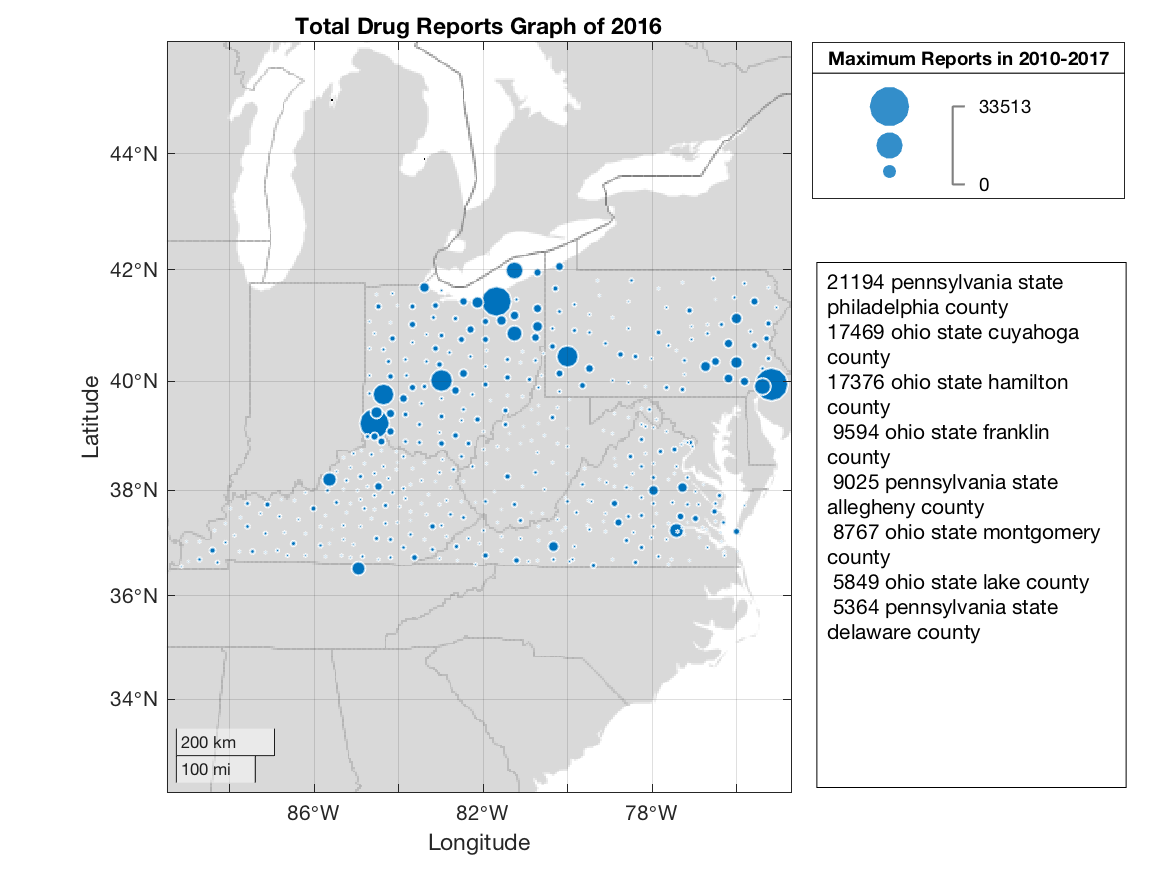
\includegraphics[width=6in]{figures/TotalDrugReportsCounty2016.png}
\caption{Total Drug Reports By County in 2016}
\label{Total Drug Reports County in 2016}
\end{figure}

\subsubsection{Preliminary analysis}
Based on the result of visualization, we can see that the number of Total Drug Reports in the four counties ----Pennsylvania State Philadelphia County,Ohio State Hamilton County,Pennsylvania State Allegheny County,Ohio State Montgomery County
----was more than 5000 in 2010-2017. The number of Total Drug Reports in Ohio State Cuyahoga County in 2010-2017 was more than 5000 in 6 years and its growth was the fastest of all counties. The statistical results of the total number of Total Drug Reports over 5000 are shown in the table below. 
% Table generated by Excel2LaTeX from sheet 'Sheet1'
% Table generated by Excel2LaTeX from sheet 'Sheet1'
\begin{table}[htbp]
  \centering
  \caption{results of the total number of Total Drug Reports over 5000}
    \begin{tabular}{cc}
    \toprule
    Value & Count \\
    \midrule
    Pennsylvania State Philadelphia County & 8 \\
    Ohio State Hamilton County & 8 \\
    Pennsylvania State Allegheny County & 8 \\
    Ohio State Montgomery County & 8 \\
    Pennsylvania State Bucks County & 3 \\
    Kentucky State Jefferson County & 2 \\
    Ohio State Cuyahoga County & 6 \\
    Ohio State Franklin County & 6 \\
    Ohio State Lake County & 2 \\
    \bottomrule
    \end{tabular}%
  \label{tab:results of the total number of Total Drug Reports over 5000}%
\end{table}%



\subsection{Model construction}
\subsubsection{Modeling}
In general, when a drug identification occurs in a county, it may affect the number of such cases in other counties. (The number of such cases may increase or decrease.) It is easy to understand that the possibility of the occurrence of such cases is closely related to the position of other county----First, when two counties are located in the same state, the one of them can easily affect the other one. (Of course, for a specific county, a county in another state can affect it as well, but in less strength.) Second, the shorter the distance between a county and another county, the greater the mutual influence they directly receive, the greater the possibility drug identifications occur at the same time in these two counties. We create matrix $G = {\left( {{g_{ij}}} \right)_{5 \times 5}}$ to describe the impact level between two counties, where ${g_{ij}}$ means the impact level of drug cases occurring in counties in the state j towards counties in state i. The farther the distance, the lower the level of influence.  We define
 \begin{equation}{g_{ij}} = \left\{ \begin{array}{l}
\frac{{\frac{1}{{{d_{ij}}}}}}{{\sum\limits_{i,j} {\frac{1}{{{d_{ij}}}}} }}{\rm{              }}i \ne j\\
1{\rm{                       }}i = j
\end{array} \right. \end{equation}
Apparently, matrix $G$ is a symmetric matrix.

At the same time the possibility of a county with a drug case affecting the number of cases in other counties is also related to the number of drug cases in the county.  Therefore we first divide the counties in each of the five states into three categories according to the number of cases in the county/the total number of cases in five states

We divide all counties in these five states into three groups:
\begin{enumerate}
  \item 	In these five states, there are some counties where no drug cases occur at specific times. We divide these counties into a separate group, denoted as group $A$.
  \item All counties different from Group $A$ are identified with drug cases at that time, but the severity of them differ from each other. We assume that the rest counties can be divided into two groups according to the severity. We define drug infected level $m$,which is the ratio between the number of cases in the county and the total number of cases in five states. The remaining counties are divided by the average of drug infected level $m$ : the counties below the average(0.0023) belong to one group, which is the moderate drug-using group, denoted Group $B$. The counties above the average belong to one group, which is the severe drug-using group, denoted Group $C$.
\end{enumerate}


For a county $s$ in state $i$:
\begin{enumerate}
  \item If county $s$ belongs to Group $A$, the number of cases in $s$ will not influence the number of cases in other counties.
  \item If county $s$ belongs to Group $B$, the number of cases in $s$ will only influence the number of cases in counties that belong to Group $A$.
  \item If county $s$ belongs to Group B, the number of cases in $s$ will only influence the number of cases in counties that belong to Group $A$.
\end{enumerate}

To simplify the problem, we need to make the following notations:
\begin{table}[H]
  \centering
  \caption{results of the total number of Total Drug Reports over 5000}
    \begin{tabular}{lp{12cm}p{12cm}p{12cm}}
    \toprule
    Value & Count \\
    \midrule
 $t$&Time\\
 
${N_{Ci}}(t)$, ${N_{Ci}}(t)$, ${N_{Ci}}(t)$ &The number of three types of counties at time $t$ in state $i$\\

${delta _B}$& The removal rate of Group $B$ counties\\

${delta _C}$& The removal rate of Group $C$ counties\\

${C_A}$& The probability that Group $C$ counties are converted into Group $A$ counties, on the condition that they are removed from Group $C$\\

${C_B}$&The probability that Group $C $counties are converted into Group $B$ counties, on the condition that they are removed from Group $C$\\

$ {b}$&The possibility that a Group $A$ county coverts into a Group $B$ county due to the influence of $B$.\\

$ {c_1}$&The possibility that a Group $B$ county covert into a Group $C$ county due to the influence of $C$.\\

$ {c_21}$&The possibility that a Group $A$ county coverts into a Group $B$ county due to the influence of $C$.\\

$ {c_22}$& The possibility that a Group $A$ county coverts into a Group $C$ county due to the influence of $C$.\\

${T_{ABi}}(t)$&The number of Group $A$ counties converted into Group $B$ counties in state $i$ at time $t$. \\

${T_{AC}}(t)$& The number of Group $A$ counties converted into Group $B$ counties in state $i$ at time $t$.\\

${T_{BC}}(t)$& The number of Group $A$ counties converted into Group $B$ counties in state $i$ at time $t$.\\
    \bottomrule
    \end{tabular}%
  \label{tab:results of the total number of Total Drug Reports over 5000}%
\end{table}%


In addition to being affected by counties with a large number of other cases, the number of cases in a county may be reduced due to restrictions imposed by national policies. This probability is related to the number of cases itself.  For the three types of counties we have defined we can see that we have a basis for dividing the three types of counties. We can think that the probability of the number of counties in any one of the counties being converted to another type of counties is a fixed number.

Now we analyze the change of the number of counties in Group $A$, $B$, $C$ separately.

${T_{ABi}}(t)$ is composed by two parts:
\begin{enumerate}
  \item The number of Group $A$ counties in the state I that are converted into Group $B$ counties by the influence of Group $B$ counties in all 5 states  
  \item The number of Class $A$ counties in the state $I$ that are converted into Group $B$ counties by the influence of Group B counties in all 5 states
\end{enumerate}

 
 \begin{equation}{T_{ABi}}(t) = \sum\limits_{j = 1}^5 {{g_{ij}}{N_{Bj}}(t){N_A}_i(t)} b + \sum\limits_{j = 1}^5 {{g_{ij}}{N_{Cj}}(t)} {N_A}_i(t){c_{21}} \end{equation}

${T_{AC}}(t)$ is the number of Group $A$ counties in the state $I$ that are converted into Group $B$ counties by the influence of Group $B$ counties in all 5 states 
                         \begin{equation}{T_{ACi}}(t) = \sum\limits_{j = 1}^5 {{g_{ij}}{N_{Cj}}(t)} {N_A}_i(t){c_{22}} \end{equation}
${T_{BC}}(t)$ is the number of Group $B$ counties in the state $I$ that are converted into Group $C$ counties by the influence of Group $C$ counties in all 5 states 
  \begin{equation}{T_{BCi}}(t) = \sum\limits_{j = 1}^5 {{g_{ij}}{N_{Cj}}(t)} {N_B}_i(t){c_1} \end{equation}
 
${\delta _B}{N_{Bi}}(t)$ ,${C_A}{\delta _C}{N_{Ci}}(t)$are the number of  Group $B$ and Group $C$ counties converted into Group A counties after they reduce the number of cases , that is, the net increase in the number of Class $A$ counties.  Consider the increase in the number of counties from $t$ to $t + \Delta t$ :
 
 \begin{equation}{N_{Ai}}(t + \Delta t) - {N_{Ai}}(t) = ({\delta _B}{N_{Bi}}(t) - {T_{ABi}}(t) - {T_{ACi}}(t) + {C_A}{\delta _C}{N_{Ci}}(t))\Delta t \end{equation}
Then we get the differential equations:
                
 \begin{equation}\frac{{d{N_{Ai}}(t)}}{{dt}} = {\delta _B}{N_{Bi}}(t) - {T_{ABi}}(t) - {T_{ACi}}(t) + {C_A}{\delta _C}{N_{Ci}}(t) \end{equation}
Similarly, we get the growth rate of Group $B$, $C$ counties
              
 \begin{equation}\left\{\begin{array}{l}
\frac{{d{N_{Ai}}(t)}}{{dt}} = {\delta _B}{N_{Bi}}(t) - {T_{ABi}}(t) - {T_{ACi}}(t) + {C_A}{\delta _C}{N_{Ci}}(t)\\
\frac{{d{N_{Bi}}(t)}}{{dt}} = {T_{ABi}}(t) - {\delta _B}{N_{Bi}}(t) - {T_{BCi}}(t) + {C_B}{\delta _C}{N_{Ci}}(t)\\
\frac{{d{N_{Ci}}(t)}}{{dt}} = {T_{BCi}}(t) - {\delta _C}{N_{Ci}}(t) + {T_{ACi}}(t)
\end{array}\right. \end{equation}
where
\begin{equation}
  {C_A} + {C_B} = 1
\end{equation}

Finally, we get the Drug Spread Model
 
 \begin{equation}\left\{ \begin{array}{l}
\frac{{d{N_{Ai}}(t)}}{{dt}} = {\delta _B}{N_{Bi}}(t) - {T_{ABi}}(t) - {T_{ACi}}(t) + {C_A}{\delta _C}{N_{Ci}}(t)\\
\frac{{d{N_{Bi}}(t)}}{{dt}} = {T_{ABi}}(t) - {\delta _B}{N_{Bi}}(t) - {T_{BCi}}(t) + {C_B}{\delta _C}{N_{Ci}}(t)\\
\frac{{d{N_{Ci}}(t)}}{{dt}} = {T_{BCi}}(t) - {\delta _C}{N_{Ci}}(t) + {T_{ACi}}(t)
\end{array} \right. \end{equation}



\subsubsection{Obtaining parameters} \label{Obtaining parameters}
From the first document we can get the number of counties in Group $A$, $B$ and $C$ in each state in 2010-2017. So we let   $\Delta t = 1$ and convert equation (1)(2) into discrete forms:
 \begin{equation}\begin{array}{l}
{N_{Ai}}(t + 1) - {N_{Ai}}(t) \approx {\delta _B}{N_{Bi}}(t) - {T_{ABi}}(t) - {T_{ACi}}(t) + {C_A}{\delta _C}{N_{Ci}}(t) \buildrel \Delta \over = {f_{i1}}\\
{N_{Bi}}(t + 1) - {N_{Bi}}(t) \approx {T_{ABi}}(t) - {\delta _B}{N_{Bi}}(t) - {T_{BCi}}(t) + {C_B}{\delta _C}{N_{Ci}}(t) \buildrel \Delta \over = {f_{i2}}\\
{N_{Ci}}(t + 1) - {N_{Ci}}(t) \approx {T_{BCi}}(t) - {\delta _C}{N_{Ci}}(t) + {T_{ACi}}(t) \buildrel \Delta \over = {f_{i3}}\\
{C_A} + {C_B} = 1{\rm{                                                             }}\,i = 1,2,3,4,5
\end{array} \end{equation}
We denote,
 \begin{equation}{r_{ij}} = \left\{ \begin{array}{l}
{[{f_{k1}} - ({N_{Ak}}(t + 1) - {N_{Ak}}(t))]_{t = {t_j}}}{\rm{            }}i = 3k + 1\\
{[{f_{k2}} - ({N_{Bk}}(t + 1) - {N_{Bk}}(t))]_{t = {t_j}}}{\rm{            }}i = 3k + 2\\
{[{f_{k3}} - ({N_{Ck}}(t + 1) - {N_{Ck}}(t))]_{t = {t_j}}}{\rm{            }}i = 3k + 3
\end{array} \right.{\rm{     }}i = 1...15,j = 1...7 \end{equation}

The ${r_{ij}}$ is called the residual which characterizes the error of the numerical fitting,  where ${t_j}$ is the value of the independent variable $t$.

To compute the parameters ${\delta _B},{\delta _C},b,{c_1},{c_{21}},{c_{22}},{C_A}$,  we use the least squares criterion to determine the value of the parameter so that the sum of the squares of the residuals is minimal.
 
 \begin{equation}R = \sum\limits_{i = 1}^{15} {\sum\limits_{j = 1}^7 {{r_{ij}}^2} }   \end{equation}
Since the values of all the parameters are in $[0,1]$, the parameters can be obtained by solving the following constraint optimization problem:
 
 \begin{equation}\begin{array}{l}
\min R = \sum\limits_{i = 1}^{15} {\sum\limits_{j = 1}^7 {{r_{ij}}^2} } \\
s.t.\,{\rm{  }}{\delta _B},{\delta _C},b,{c_1},{c_{21}},{c_{22}},{C_A} \in [0,1]
\end{array} \end{equation}
Using Matlab function "fmincon()"\upcite{higham2016matlab}, we can compute the estimated value of all parameters:
 
 \begin{equation}\left\{ \begin{array}{l}
{\delta _B} = 0.0365\\
{\delta _C} = 0.0277\\
b = 0.0031\\
{C_1} = 0.0042\\
{C_{21}} = 1.0566 \times {10^{ - 8}}\\
{C_{22}} = 1.1231 \times {10^{ - 9}}\\
{C_B} = 1\\
{C_A} = 0
\end{array} \right. \end{equation}

In this model, each parameter has its practical meaning, so we can recognize the way and features of drug cases “spreading” between different states.

For the counties in Group $C$, there is a possibility of ${\delta _C} = 0.0277$ that counties are transformed into other types of counties. More accurately, there is a possibility of ${\delta _C} \times {C_B} = 0.0277$ that Group C counties are transformed into Group $B$ counties, which cannot be directly converted into Group $A$ counties, however. For Group $B$ counties, there is a possibility of ${\delta _B} = 0.0365$ that they are transformed into Group $A$ counties.

The number of counties in each of the three categories of states is related to the number of counties in the three states of the five states since the increase in the number of cases per county is affected by the number of cases in other counties.  For example, for Kentucky, the number of Group $A$ counties converted into Group $B$ counties is
 
 \begin{equation}\begin{array}{l}
{T_{AB1}}(t) = \sum\limits_{j = 1}^5 {{g_{1j}}{N_{Bj}}(t){N_A}_1(t)} b + \sum\limits_{j = 1}^5 {{g_{1j}}{N_{Cj}}(t)} {N_A}_1(t){c_{21}}\\
{\rm{          }} = \sum\limits_{j = 1}^5 {{g_{1j}}{N_{Bj}}(t){N_A}_1(t)}  \times 0.0031 + \sum\limits_{j = 1}^5 {{g_{1j}}{N_{Cj}}(t)} {N_A}_1(t) \times 1.0566 \times {10^{ - 8}}
\end{array} \end{equation}
The number of Group $A$ counties converted into Group $C$ counties is  
 \begin{equation}{T_{AC1}}(t) = \sum\limits_{j = 1}^5 {{g_{1j}}{N_{Cj}}(t)} {N_A}_1(t) \times 1.1231 \times {10^{ - 9}} \end{equation}
The number of Group $B$ counties converted into Group $C$ counties is  
 \begin{equation}{T_{BC1}}(t) = \sum\limits_{j = 1}^5 {{g_{1j}}{N_{Cj}}(t)} {N_B}_1(t) \times 0.0042 \end{equation}
 
\subsection{Solution of model}
\subsubsection{Trend of future}
We have obtained the values of the given 7 parameters approximated by the data in "MCM\_NF\\LIS\_Data.xlsx". Now we get the linear ordinary differential equations. We regard the data in 2010 as the initial value condition, and use the function "dsolve()" in Matlab\upcite{higham2016matlab} to solve the differential equations, so that we get a set of functions of the number and time of each of the three groups in each state (Due to the limitation of the paper’s space, the solutions is shown in the appendix.). We let $t\in [0,50]$ ,and draw the figures of the functions.

\begin{figure}[H]
\centering
\begin{minipage}[t]{0.45\textwidth}
\centering
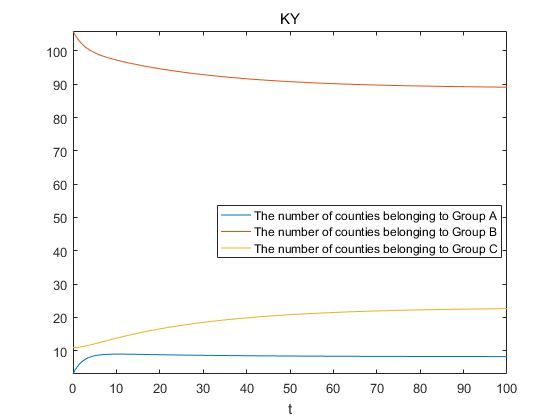
\includegraphics[width=3.2in]{figures/picture/KY_1.jpg}
\caption{KY 1}
\label{KY 1}
\end{minipage}
\hfill
\begin{minipage}[t]{0.45\textwidth}
\centering
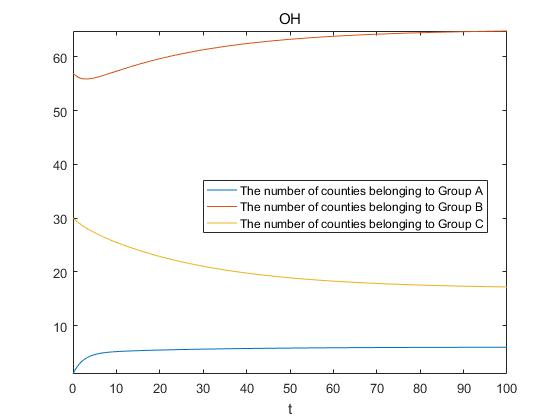
\includegraphics[width=3.2in]{figures/picture/OH_1.jpg}
\caption{OH 1}
\label{OH 1}
\end{minipage}
\end{figure}

\begin{figure}[H]
\centering
\begin{minipage}[t]{0.45\textwidth}
\centering
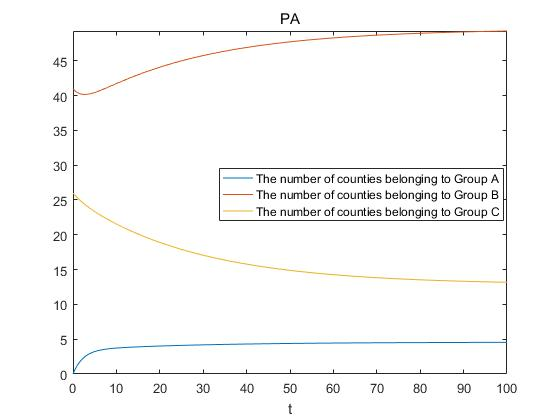
\includegraphics[width=3.2in]{figures/picture/PA_1.jpg}
\caption{PA 1}
\label{PA 1}
\end{minipage}
\hfill
\begin{minipage}[t]{0.45\textwidth}
\centering
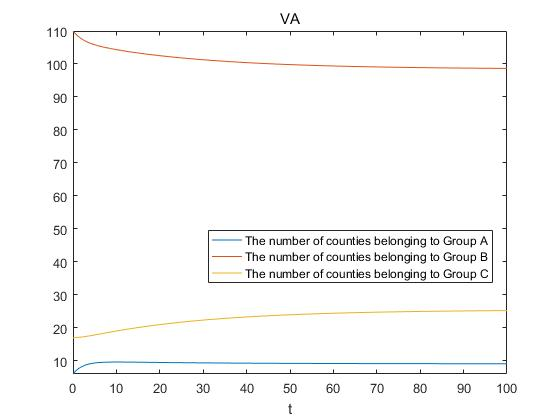
\includegraphics[width=3.2in]{figures/picture/VA_1.jpg}
\caption{VA 1}
\label{VA 1}
\end{minipage}
\end{figure}

\begin{figure}[H]
\centering
\begin{minipage}[t]{0.45\textwidth}
\centering
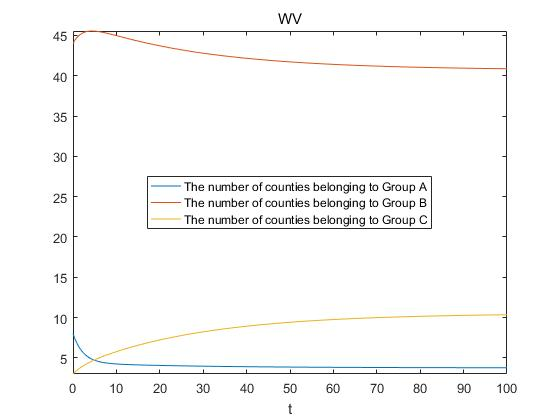
\includegraphics[width=3.2in]{figures/picture/WV_1.jpg}
\caption{WV 1}
\label{WV 1}
\end{minipage}
\hfill
\begin{minipage}[t]{0.45\textwidth}
\end{minipage}
\end{figure}

From the five figures above, we can find that
\begin{enumerate}
  \item In the next 40 years the number of Group $C$ counties in Kentucky, Virginia and West Virginia has a certain increase about 10\%; The number of Group $A$ counties remains basically the same.  The number of Group $B$ counties has decreased. As the number of counties in each state unchanged, the decrease in the number of Group $B$ counties approximately equals to the increase in the number of Group $C$ counties. For Ohio and Pennsylvania, the number of Group $A$ counties remains basically the same, but the number of Group $C$ counties is decreasing and the number of Group $B$ counties is increasing. 

We can roughly understand that without policy interventions, some of the severe drug-using counties in Ohio and Pennsylvania will be converted to moderate drug-using counties. Some of the moderate drug-using counties in Kentucky, Virginia and West Virginia will be transformed into severe drug-using counties. Therefore, the government should focus on drug cases in Kentucky Virginia and West Virginia. 
\item The number of counties in the three groups of five states tends to be stable over time. Since the number of counties in the three categories is directly related to the number of drug cases in each county, we have reason to believe that when the number of three groups of counties in a state becomes stable, the drug identification has reached the threshold level. From the above five figures we found that Virginia was the first to reach a stable state and it reached a steady state in the 60th year. Therefore, we can consider that in the 60th year ---that is, the year 2070---the drug identification in Virginia reached a threshold level.
\end{enumerate}

\subsubsection{Finding where Heroin started}
In Section \ref{Obtaining parameters} , We have calculated the number of Group $A$, $B$ and $C$ counties in each state as a function of time according to the number and proportion of all drug cases.  Next we counted the number of heroin cases in each county in the first document and the number of counties $A$, $B$ and $C$ classified by number and proportion of heroin cases in each state in 2010-2017.Here we get the optimal value of all parameters:
\begin{equation}
	\left\{ \begin{array}{l}
{\delta _B} = 0.0698\\
{\delta _C} = 0.2259\\
b = 0.0024\\
{C_1} = 0.0028\\
{C_{21}} = 0.0066\\
{C_{22}} = 2.1404 \times {10^{ - 6}}\\
{C_B} = 1\\
{C_A} = 0
\end{array} \right.
\end{equation}

Then we use Matlab function to solve the corresponding ordinary differential equations to obtain the function of the number and time of each county in each of the three groups of each state\upcite{higham2016matlab}. We let $ \in [ - 10,20]$, and get the figures of the functions:

\begin{figure}[H]
\centering
\begin{minipage}[t]{0.45\textwidth}
\centering
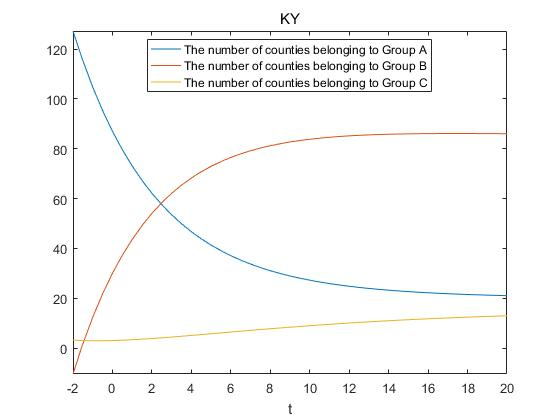
\includegraphics[width=3.2in]{figures/picture/KY_2.jpg}
\caption{KY 2}
\label{KY 2}
\end{minipage}
\hfill
\begin{minipage}[t]{0.45\textwidth}
\centering
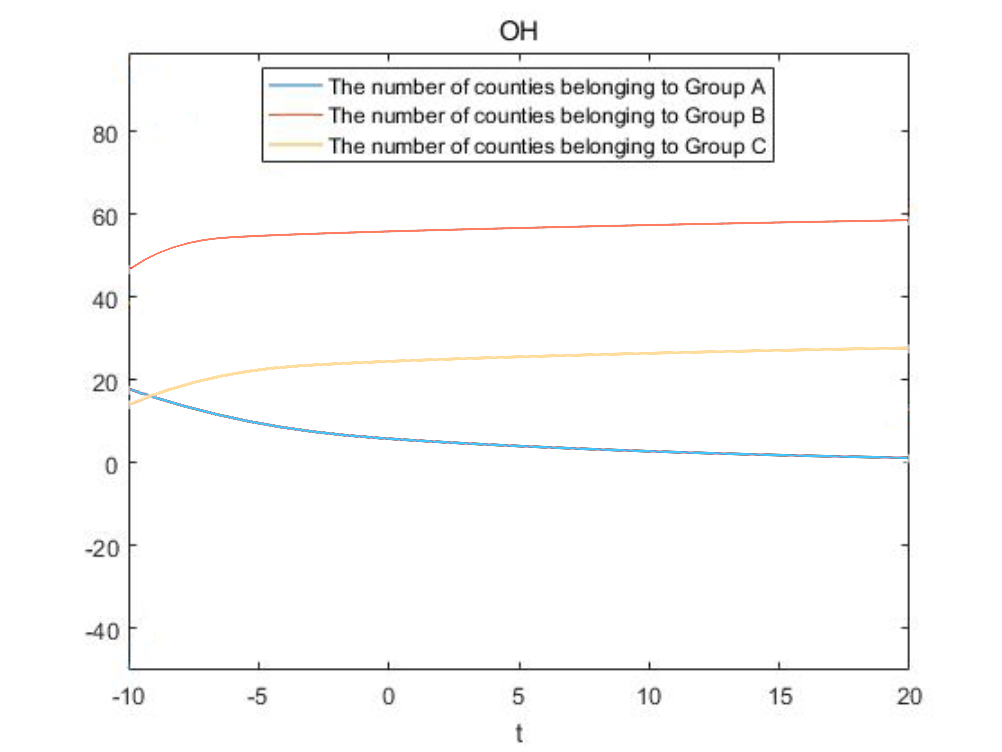
\includegraphics[width=3.2in]{figures/picture/OH_2.jpg}
\caption{OH 2}
\label{OH 2}
\end{minipage}
\end{figure}

\begin{figure}[H]
\centering
\begin{minipage}[t]{0.45\textwidth}
\centering
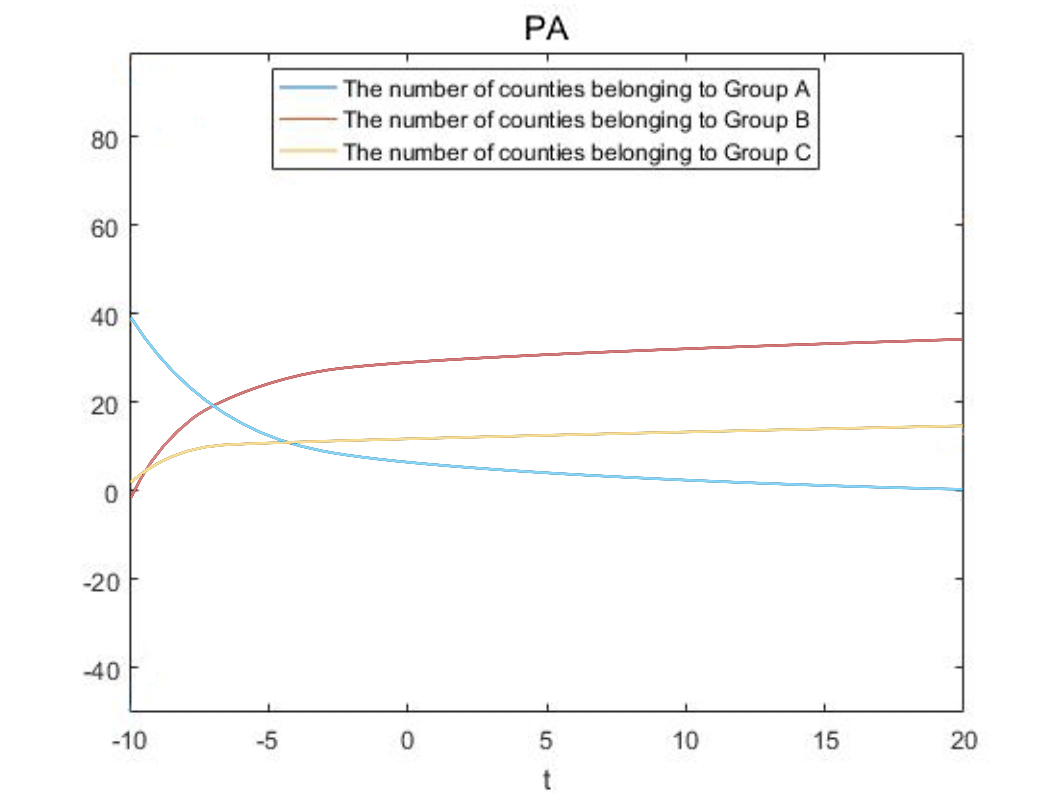
\includegraphics[width=3.2in]{figures/picture/PA_2.jpg}
\caption{PA 2}
\label{PA 2}
\end{minipage}
\hfill
\begin{minipage}[t]{0.45\textwidth}
\centering
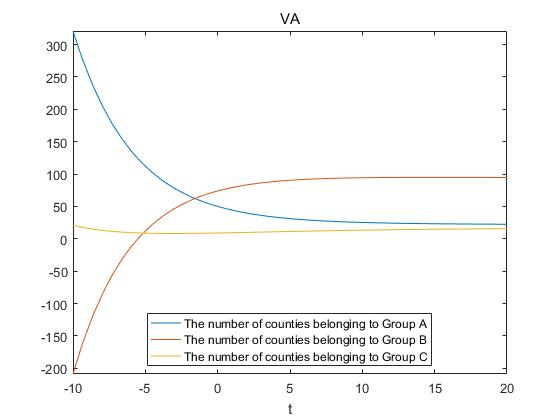
\includegraphics[width=3.2in]{figures/picture/VA_2.jpg}
\caption{VA 2}
\label{VA 2}
\end{minipage}
\end{figure}

\begin{figure}[H]
\centering
\begin{minipage}[t]{0.45\textwidth}
\centering
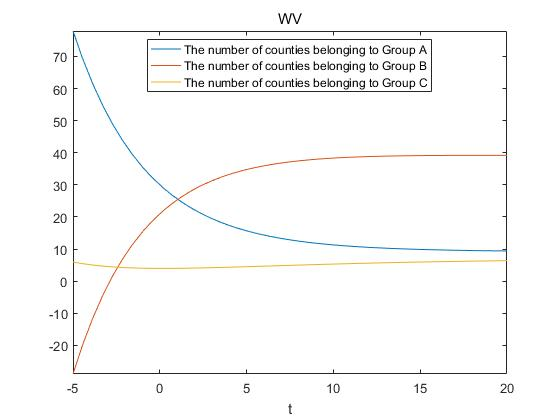
\includegraphics[width=3.2in]{figures/picture/WV_2.jpg}
\caption{WV 2}
\label{WV 2}
\end{minipage}
\hfill
\begin{minipage}[t]{0.45\textwidth}
\end{minipage}
\end{figure}


Set 2010 at $t = 0$ the image shows that the timing of heroin identification cases in Kentucky Pennsylvania Virginia and West Virginia is about -2, -10, -5, -3, while for Ohio, at $t = -10$ the three groups of counties still have a relatively large number so it can be considered that Ohio first began to appear heroin cases.  At the same time we can also see in the image that the number of counties in the three states of the five states tends to be stable over time. From the analysis in section 1.2.1 there is a threshold level for drug identification and even we can directly conclude that In the seventh year---that is, the year 2017--- drug identification in Virginia reached a threshold level.













\section{Selection of socio-economic factors}
Since the given data is spatio-temporal data the data dimension is extremely large, we should reduce the dimensionality of the data and extract useful data. 

\subsection{Preliminary cleaning and screening variables \\\small{(Take “ACS\_10\_5YR\_DP02.zip” data as an example)}}

\subsubsection{Eliminate duplicate social data indicators}
In the socio-economic indicator data of “ACS\_10\_5YR\_DP02\_with\_ann.csv”, there are 464*596 data (the number of counties* the number of social and economic indicators). According to the data given by the topic we know the abbreviations of each variable as follows.

% Table generated by Excel2LaTeX from sheet 'Sheet1'
\begin{table}[htbp]
  \centering
  \caption{Meanings of abbreviations}
    \begin{tabular}{cc}
    \toprule
    Abbreviations & Meanings \\
    \midrule
    HC\_01 & Estimate\\
    HC\_02 & Margin of Error \\
    HC\_03 & Percent \\
    HC\_04 & Percent Margin of Error \\
    VC\_XX & Types of economic data \\
    \bottomrule
    \end{tabular}%
  \label{tab:abbreviations}%
\end{table}%

It can be seen that there is only a dimensional difference between HC\_01 and HC\_03 ,and HC\_02 and HC\_04 ,which are repeated social data indicators. Only two of them can be selected. The data gap entries in HC\_03 and HC\_04 are more than HC\_01 and HC\_02 , so we only considers HC\_01 and HC\_02 and the data volume drops to 464*298.

\subsubsection{Processing missing indicators}

According to “ACS\_10\_5YR\_DP02.txt”, we know that the distribution and types of missing data in the socioeconomic indicator data are as follows.
% Table generated by Excel2LaTeX from sheet 'Sheet1'
\begin{table}[htbp]
  \centering
  \caption{Distribution and types of missing data in the socioeconomic indicator}
    \begin{tabular}{p{5em}p{13.915em}p{11.835em}}
    \toprule
    Data Type & Possible Missing Data Type & Handle Way \\
    \midrule
    HC\_01 & (X) & Delete \\
    HC\_02 & (X)\textbackslash{}*****\textbackslash{}*** & Delete\textbackslash{}Ignore\textbackslash{}Ignore \\
    HC\_03 & (X)\textbackslash{}- & Delete\textbackslash{}Replace with 0 \\
    HC\_04 & (X)\textbackslash{}** & Delete\textbackslash{}Replace with 100 \\
    \bottomrule
    \end{tabular}%
  \label{tab:addlabel}%
\end{table}%


\begin{itemize}
  \item (X)data
It refers to an entirely missing column of data. So we directly eliminate this type of data.

\item *****/*** data
It refers to individual missing data. This error only occurs with HC\_02. Since we do not use this data, it is ignored.

\item - data
It refers to individual missing data. The reason for this is that the amount of data is small so we replace it directly with 0.

\item ** data
It refers to individual missing data. The reason for the occurrence is that the sample observation value or the sample observation value is too small to calculate the standard error. The data standard error is unknown and may be taken as 100 which is classified as a large error indicator.
\end{itemize}

\subsubsection{Excluding the counties that did not appear in the data}

In the previous Part A, the number of counties is 445.  In “ACS\_10\_5YR\_DP02\_with\_ann.csv” the number of counties is 464. Since we analyze the socio-economic indicator data below we will use the data of each county in each year as a sample to carry out LASSO regression to ensure the county sample.  The dimensions are the same and we have removed the counties that did not appear in the first question data here.





\subsubsection{Eliminate indicators with large errors}


 \begin{figure}[H]
\centering
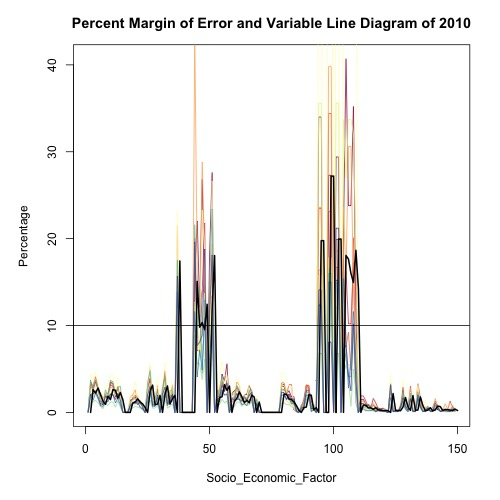
\includegraphics[width=3.2in]{figures/PercentMarginErrorDataGraphVariable2010.jpeg}
\caption{Percent Margin Error Data and Variable Graph 2010 \protect\footnotemark}
\label{Percent Margin Error Data and Variable Graph 2010}

\end{figure}
\footnotetext{Caption: The color of the same color line is the error percentage distribution line of each social and economic indicator of a single county. The black line is the error percentage distribution line of all the social and economic indicators of all counties. The horizontal line of 10\% is the threshold line for large error indicators.} 
 
Based on the percentage error data in the socioeconomic indicator data, we plot the upper graph for all 149 indicator variables.  According to the image we can see that the error percentage of most social and economic indicators is below 10\%. In order to ensure the accuracy of the subsequent screening variables we removed the indicator with a large percentage error (>10\%) and the data volume decreased.  The data volume drops to 464*298.

\subsection{Dimension reduction and variables filtering by LASSO regression\\\small{(Take “ACS\_10\_5YR\_DP02.zip” data as an example)}}

After our initial screening of the data the total amount of data is still large, although the data dimension has declined. Moreover the socioeconomic indicator data is spatiotemporal data and there is likely to be serious multicollinearity between the data. Therefore in order to screen out important socio-economic indicators we need to further refine the data.
\subsubsection{ Multicollinearity test}
First we test the multicollinearity\upcite{mansfield1982detecting} of the data.
\begin{itemize}
  \item \textbf{Calculate the rank of the matrix}\\
Using R software we can calculate the rank of the socioeconomic indicator data matrix X and get R(X)=98.  Since the dimension of the socioeconomic indicator data matrix X is 445*131 the socioeconomic indicator data matrix is not full rank, indicating that $X_i$ can be represented by other linear combinations of $X_j$ that is there may be collinearity.
\item \textbf{Calculate condition number}\\
Since matrix X may have collinearity but not complete linear correlation, we calculate the condition number kappa(X). 

\begin{itemize}
  \item If k<100 indicates that the degree of collinearity is small;
  \item If 100<k<1000 there is more multi-colinearity;
  \item If k>1000 there is severe multicollinearity.
\end{itemize}

We calculate the condition number of X as Inf >> 1000 and consider that X has very serious multicollinearity.  Therefore we need to build a model that meets the following two requirements.
\begin{enumerate}
  \item Eliminate the multicollinearity of data
  \item Screen out the factors related to the high drug abuse rate in the socioeconomic indicator data.
\end{enumerate}
\end{itemize}



                                                
\subsubsection{Cross validation and Lasso Regression}

We use the “glmnet” package in R to regress the data\upcite{james2013introduction}. The parameter $\lambda$ normalized in the glmnet package is in $[0,1]$ and the standardization formula is as follows: 


\begin{equation}
  \hat{\lambda} = −log(\lambda), \lambda \in [0, 1] 
\end{equation}
    

In order to estimate the parameters of the model using LASSO first we select 100 values of $\lambda$ and build 100 LASSO regression models.  Where the distribution of $\lambda$ is as shown in the figure:
\begin{figure}[H]
\centering
\begin{minipage}[t]{0.45\textwidth}
\centering
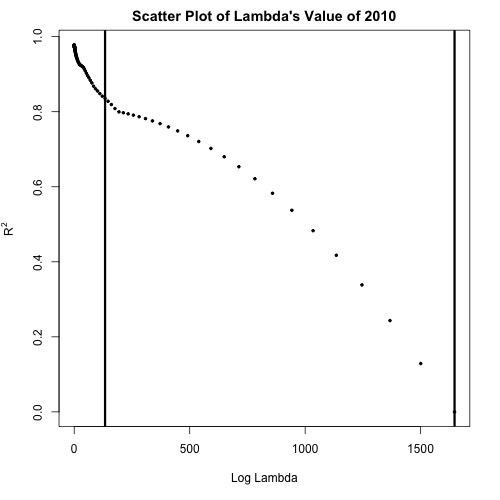
\includegraphics[width=3.2in]{figures/SelectedLambdaCorrespondingRegressR2Graphof2010}
\caption{Selected Lambda Corresponding RegressnR2nGraph of 2010}
\label{WV 2}
\end{minipage}
\hfill
\begin{minipage}[t]{0.45\textwidth}
\centering
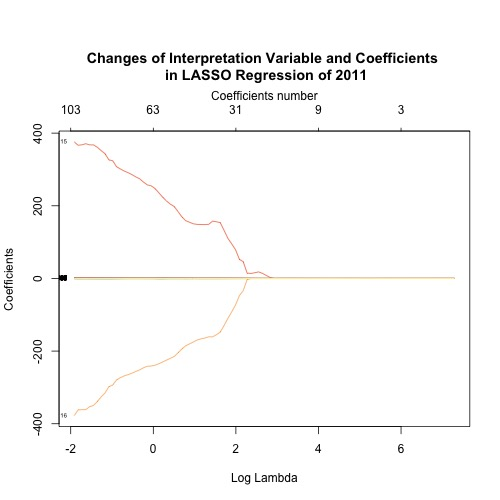
\includegraphics[width=3.2in]{figures/ChangesofInterpretationVariableandCoefficientsinLASSORegressionof2011.jpeg}
\caption{Changes of Interpretation Variable and Coefficients in LASSO Regression of 2010}
\label{Changes of Interpretation Variable and Coefficients in LASSO Regression of 2010}
\end{minipage}
\end{figure}

  
By taking the 100 sets of $\lambda$ values we selected into the LASSO model we get 100 sets of regression equations.  To understand our model intuitively we have drawn Figure 3.2. Each curve in the graph represents the trajectory of the coefficient of each independent variable. The ordinate is the value of the coefficient the lower abscissa is log($\lambda$) and the upper abscissa is the number of non-zero coefficients in the model at this time. We can see that the non-zero coefficient at the beginning of $\lambda$ is smaller as the value of $\lambda$ becomes larger and eventually all coefficients converge to zero.

The selection of parameter $\lambda$ for the LASSO regression model is important when selecting the LASSO parameter $\lambda$ artificially:

\begin{enumerate}
  \item If $\lambda$ is chosen too large, all parameters w will be minimized resulting in under-fitting;
  \item If $\lambda$ is chosen too small, it will lead to improper resolution of the overfitting problem;
  \item Artificially selecting the $\lambda$ value is subjective and not easy to operate.
\end{enumerate}

To solve these problems we cross validation to choose the optimal $\lambda$ value.

\subsubsection{Selecting $\lambda$ by using 10-fold cross-validation} 
We use 10 cross-validation to perform cross-check on the 100 $\lambda$ values in the previous section. The results are shown in the following figure.

\begin{figure}[H]
\centering
\begin{minipage}[t]{0.45\textwidth}
\centering
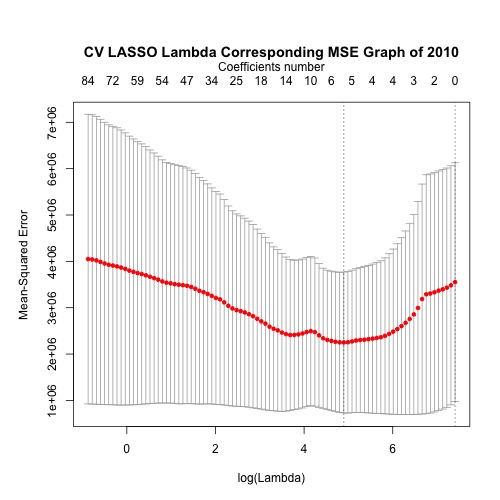
\includegraphics[width=3.2in]{figures/CVLASSOLambdaCorrespondingMSEGraphof2010.jpeg}
\caption{CV LASSO Lambda Corresponding MSE Graph of 2010}
\label{CVLASSOLambdaCorrespondingMSEGraphof2010}
\end{minipage}
\hfill
\begin{minipage}[t]{0.45\textwidth}
\centering
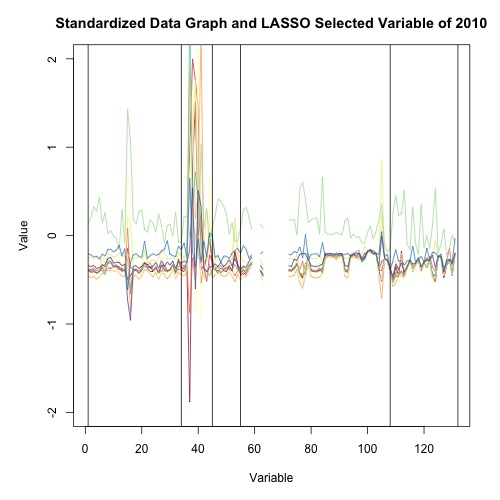
\includegraphics[width=3.2in]{figures/StandardDataLASSOVariableof2010.jpeg}
\caption{Standard Data LASSO Variable of 2010}
\label{StandardDataLASSOVariableof2010}
\end{minipage}
\end{figure}
 
In Figure \ref{CVLASSOLambdaCorrespondingMSEGraphof2010}, the red scatter is the scatter plot for the cross-check. The horizontal axis is log$\lambda$ and the vertical axis is the mean square error. The upper and lower bounds of the standard deviation for each point are also drawn.  The top word count of the graph represents the number of non-zero coefficients and the two vertical dashed lines are the selected $\lambda$ after the cross-check.  Among them a dotted line refers to the value of the interactive test that minimizes the mean square error (MSE) $\lambda$ and the other dotted line is the $\lambda$ value that is one standard deviation from the minimum mean square error.

\subsubsection{Result analysis and prediction}
We select the $\lambda$ value with the smallest mean square error (MSE) from 100 $\lambda$ by cross validation and then get the corresponding regression model.  The $\lambda$ value selected here selects 59 explanatory variables and the coefficient positions of each are shown in Figure \ref{StandardDataLASSOVariableof2010}. The coefficients of each explanatory variable are shown in the Appendix.
 

\subsubsection{filtering variables}
For the variables obtained from the application of LASSO regression in 2010-2016, we obtained all explanatory variables that occurred more than 3 times in 7 years as shown in the following table.

 %Table generated by Excel2LaTeX from sheet 'Sheet1'
\begin{table}[htbp]
  \centering
  \small
  \caption{Explanatory variables that occurred more than 3 times in 7 years}
    \begin{tabularx}{\textwidth}{llX}
    \toprule
    Abbr & Count & Meaning \\
    \midrule
    HC01\_VC10 & 5 & HOUSEHOLDS BY TYPE - Total households - Family households (families) - Female householder, no husband present, family \\
    HC01\_VC122 & 5 & RESIDENCE 1 YEAR AGO - Population 1 year and over - Different house in the U.S. - Same county \\
    HC01\_VC66 & 5 & GRANDPARENTS - Number of grandparents living with own grandchildren under 18 years - Years responsible for grandchildren - 1 or 2 years \\
    HC01\_VC188 & 4 & ANCESTRY - Total population - Czech \\
    HC01\_VC190 & 4 & ANCESTRY - Total population - Dutch \\
    HC01\_VC204 & 4 & ANCESTRY - Total population - Scotch-Irish \\
    HC01\_VC54 & 4 & FERTILITY - Number of women 15 to 50 years old who had a birth in the past 12 months - Unmarried women (widowed, divorced, and never married) - Per 1,000 unmarried women \\
    HC01\_VC87 & 4 & EDUCATIONAL ATTAINMENT - Population 25 years and over - 9th to 12th grade, no diploma \\
    HC01\_VC13 & 3 & HOUSEHOLDS BY TYPE - Total households - Nonfamily households - Householder living alone \\
    HC01\_VC185 & 3 & ANCESTRY - Total population \\
    HC01\_VC43 & 3 & MARITAL STATUS - Females 15 years and over \\
    HC01\_VC52 & 3 & FERTILITY - Number of women 15 to 50 years old who had a birth in the past 12 months \\
    HC01\_VC86 & 3 & EDUCATIONAL ATTAINMENT - Population 25 years and over - Less than 9th grade \\
    \bottomrule
    \end{tabularx}%
  \label{tab:addlabel}%
\end{table}%

\section{Modifying Drug Spread Model}
\subsection{Modified Drug Spread Model}
In Drug Spread Model we constructed eight parameters to characterize the changes in each county of each state and assumed that they have no relationship with time and then the optimal parameters were obtained from the actual discrete data of 2010-2018.  However, in fact, due to the different objective conditions such as national policy each year, these parameters may change with time. Therefore the model needs to be modified, which means correction functions ${\varepsilon _i}(t)$ are added based on the original parameter data (since ${C_A} + {C_B} = 1$, we only consider the modification of the 7 parameters) the modification of the Drug Spread Model is transformed into solving the specific form of the correction function ${\varepsilon _i}(t)$.

In past section we got a series of indicators that have a significant impact on the number of drug cases in the county. We selected two indicators that have a significant impact on the number of drug cases in the county each year: the number of men who did not have a junior high school diploma at the age of 25 (EDUCATIONAL ATTAINMENT - High school graduate (includes equivalency) EDUCATIONAL ATTAINMENT - 9th to 12th grade no diploma)and the number of unmarried women with children.  Moreover it is available from section 2.1 that in a statistical point of view, the number of drug cases in each county is linear with the two indicators and it can be considered that the two indicators are independent of each other.

We denote ${M_{A1}}(t)$ ratio of the sum of the first indicator(the number of men who did not have a junior high school diploma at the age of 25) of all Group A counties to the sum of the first indicator of all counties at time $t$.

Similarly defined variable${M_{A2}}(t)$, ${M_{B1}}(t)$, ${M_{B2}}(t)$, ${M_{C1}}(t)$, ${M_{C2}}(t)$.

First ,we convert the discrete variables into continuous variables:${M_{A1}}(t)$, ${M_{A2}}(t)$, ${M_{B1}}(t)$, ${M_{B2}}(t)$, ${M_{C1}}(t)$, ${M_{C2}}(t)$ are discrete variables,We first use the known set of discrete values to do Newton interpolation on $t$ separately to get the corresponding continuous function ${M_{A1}}(t)$, ${M_{A2}}(t)$, ${M_{B1}}(t)$, ${M_{B2}}(t)$, ${M_{C1}}(t)$, ${M_{C2}}(t)$.(All functions are listed in the Appendix.)

Then, since the eight parameters we construct is directly related to the number of drug cases in each county, we have reason to think that the correction functions a linear combination of two index functions for the sake of convenience. More specifically ,for example, the correction function for parameter ${delta _B}$---the removal rate of Group B counties--- is a linear combination of  
%${M_{B1}}(t)$,${M_{B2}}(t)$ ,which means${\varepsilon _1}(t) = {k_{11}}{M_{B1}}(t) + {k_{12}}{M_{B2}}(t)$.  For another example for parameter $b$ --- The possibility that a Group $A$ county coverts into a Group $B$ county due to the influence 
%of $B$---the correction function is a linear combination of ${M_{A1}}(t)$,$M_{A1}}(t)$, which means${\varepsilon _3}(t) = {k_{31}}{M_{A1}}(t) + {k_{32}}{M_{A2}}(t)$ . 
%Similarly, the parameters can be corrected to

\begin{equation}
	\begin{array}{l}
{\delta _B}^\prime  = 0.0365 + {k_{11}}{M_{B1}}(t) + {k_{12}}{M_{B2}}(t)\\
{\delta _C}^\prime  = 0.0277 + {k_{21}}{M_{C1}}(t) + {k_{22}}{M_{C2}}(t)\\
b' = 0.0031 + {k_{31}}{M_{A1}}(t) + {k_{32}}{M_{A2}}(t)\\
{C_1}^\prime  = 0.0042 + {k_{41}}{M_{B1}}(t) + {k_{42}}{M_{B2}}(t)\\
{C_{21}}^\prime  = 1.0566 \times {10^{ - 8}} + {k_{51}}{M_{A1}}(t) + {k_{52}}{M_{A2}}(t)\\
{C_{22}}^\prime  = 1.1231 \times {10^{ - 9}} + {k_{61}}{M_{A1}}(t) + {k_{62}}{M_{A2}}(t)\\
{C_B}^\prime  = 1 + {k_{71}}{M_{C1}}(t) + {k_{72}}{M_{C2}}(t)
\end{array}
\end{equation}
%
%
%
\subsection{Computing parameters}
In past section , we use the numerical differentiation to replace the derivative value at that moment approximate equation (1)(2) to discrete form and then solve the optimization problem of inequality constraint to get the value of the parameter.  In order to find the value of a set of parameters we can also do the above processing on the modified model YYYY. It is worth noting that the optimization problem with the sum of squared residuals as the objective function is unconstrained.  Solving an unconstrained optimization problem yields a set of optimal parameters and the parameters are corrected to

	

\begin{equation}\begin{array}{l}
{\delta _B}^\prime  = 0.0365 + 0.0209{M_{B1}}(t) - 0.0076{M_{B2}}(t)\\
{\delta _C}^\prime  = 0.0277 + 1.1326{M_{C1}}(t) + 0.0967{M_{C2}}(t)\\
b' = 0.0031 + 0.9846{M_{A1}}(t) + 1.2254{M_{A2}}(t)\\
{C_1}^\prime  = 0.0042 - 0.0014{M_{B1}}(t) + 2.8972 \times {10^{ - 4}} \times {M_{B2}}(t)\\
{C_{21}}^\prime  = 1.0566 \times {10^{ - 8}} + 2.0984 \times {10^{ - 4}} \times {M_{A1}}(t) + 0.0045{M_{A2}}(t)\\
{C_{22}}^\prime  = 1.1231 \times {10^{ - 9}} + 3.1876 \times {10^{ - 4}} \times {M_{A1}}(t) - 5.0832 \times {10^{ - 4}} \times {M_{A2}}(t)\\
{C_B}^\prime  = 1 - 0.0038{M_{C1}}(t) - 0.0142{M_{C2}}(t)
\end{array}\end{equation}
The Modified Drug Spread Model is:
\begin{equation}\begin{array}{l}
{T_{ABi}}(t) = \sum\limits_{j = 1}^5 {{g_{ij}}{N_{Bj}}(t){N_A}_i(t)} b' + \sum\limits_{j = 1}^5 {{g_{ij}}{N_{Cj}}(t)} {N_A}_i(t){c_{21}}^\prime \\
{T_{ACi}}(t) = \sum\limits_{j = 1}^5 {{g_{ij}}{N_{Cj}}(t)} {N_A}_i(t){c_{22}}^\prime \\
{T_{BCi}}(t) = \sum\limits_{j = 1}^5 {{g_{ij}}{N_{Cj}}(t)} {N_B}_i(t){c_1}^\prime \\
\frac{{d{N_{Ai}}(t)}}{{dt}} = {\delta _B}^\prime {N_{Bi}}(t) - {T_{ABi}}(t) - {T_{ACi}}(t) + {C_A}^\prime {\delta _C}^\prime {N_{Ci}}(t)\\
\frac{{d{N_{Bi}}(t)}}{{dt}} = {T_{ABi}}(t) - {\delta _B}^\prime {N_{Bi}}(t) - {T_{BCi}}(t) + {C_B}^\prime {\delta _C}^\prime {N_{Ci}}(t)\\
\frac{{d{N_{Ci}}(t)}}{{dt}} = {T_{BCi}}(t) - {\delta _C}^\prime {N_{Ci}}(t) + {T_{ACi}}(t)\\
{C_A}^\prime  + {C_B}^\prime  = 1\\
i = 1,2,3,4,5
\end{array}\end{equation}

%
%

\section{Strategies to deal with the drug crisis}
Based on our research on socioeconomic data and the number of drug cases we have obtained 13 factors that may be closely related to the number of drug cases.  If you want to reduce the rate of drug abuse you can try to consider the development of relevant policies and laws and regulations from some aspects.  On the other hand considering the two indicators involved in the revised model we have finally determined a strategy that is easy to implement increase the investment in education.

\subsection{Use model to test the feasibility of strategies}
Suppose the government invests a certain amount each year in 2010-2017 which reduces the number of people who have no junior high school diplomas over 25 years old in each county to 80\% ,that is in Modified Drug Spread Model , ${M_{A1}}(t)$, ${M_{A2}}(t)$, ${M_{B1}}(t)$, ${M_{B2}}(t)$ reduce to 80\% . Then according to section 2.2.1, the parameters of the  model are corrected to 
\begin{equation}{\delta _B}^{\prime \prime },{\delta _C}^{\prime \prime },{b^{\prime \prime }},{C_1}^{\prime \prime },{C_{21}}^{\prime \prime },{C_{22}}^{\prime \prime },{C_B}^{\prime \prime }\end{equation}. Substituting into the system of ordinary differential equations, we find the function of the number of different counties in five states over time under the policy implementation and compared it with that before the implementation. It can be clearly found that after the implementation of the policy the number of counties in each of Group $B$ and $C$ in almost every integer time in each state has a different degree of decline compared to the implementation of the policy that is the total number of drug cases, compared to the decline before the implementation of the policy, which also illustrates the feasibility of our proposed policy.
\subsection{Determine the parameter boundaries on which the policy depends}
Suppose the government invests a certain amount each year in 2010-2017 reducing the number of people in each county who are over 25 years old without a junior high school diploma to the original $k$ times, that is in Modified Drug Spread Model , 
${M_{A1}}(t)$, ${M_{A2}}(t)$, ${M_{B1}}(t)$, ${M_{B2}}(t)$ reduce to $k$ times. Substituting into the system of ordinary differential equations and the parameters of the  model are corrected 
to ${\delta _B}^{\prime \prime \prime },{\delta _C}^{\prime \prime \prime },{b^{\prime \prime \prime }},{C_1}^{\prime \prime \prime },{C_{21}}^{\prime \prime \prime },{C_{22}}^{\prime \prime \prime },{C_B}^{\prime \prime \prime }$ 
and get the solutions${N_{Ai}}{(t)^{\prime \prime \prime }},{N_{Bi}}{(t)^{\prime \prime \prime }}$,
${N_{Ci}}{(t)^{\prime \prime \prime }}$. We denote solutions before the policy implementation ${N_{Ai}}(t), {N_{Bi}}(t),{N_{Ci}}(t)$.
\begin{equation}
	f(k) = \sum\limits_{i = 1}^5 {\sum\limits_{t = 0}^7 {{N_{Bi}}(t)''' + {N_{Ci}}(t)''' - } {N_{Bi}}(t) - {N_{Ci}}(t)} 
\end{equation} 
reflects the change before and after policy implantation.We only need to solve the following optimization problem:
\begin{equation}\begin{array}{l}
\max f(k) = \sum\limits_{i = 1}^5 {\sum\limits_{t = 0}^7 {{N_{Bi}}(t)''' + {N_{Ci}}(t)''' - } {N_{Bi}}(t) - {N_{Ci}}(t)} \\
s.t.\left\{ \begin{array}{l}
0 < k < 1\\
f(k) < 0
\end{array} \right.
\end{array}\end{equation}
And we get $k=0.854$. That is to say, in 2010-2017 if the government increased investment in education the number of people in each county who did not have a junior high school diploma over 25 years old would be reduced to the original k times. As long as $k \in (0,0.854)$,  the policy is feasible.


\newpage
\section{Memorandum}
\textbf{
TO:The Chief Administrator, DEA/NFLIS Database\\
FROM:MCM Team\\
DATE:January 29, 2019\\
SUBJECT:Significant Insights and Results from Modeling}\\
We found many interesting phenomena in our modeling process.
\begin{enumerate}
  \item Based on our statistical results we can see that the distribution of drug incidents in five states is mainly concentrated near the Great Lakes (Ohio) and the US East Coast (Pennsylvania).
% Table generated by Excel2LaTeX from sheet 'Sheet1'
\begin{table}[htbp]
  \centering
  \caption{Distribution of drug incidents}
    \begin{tabular}{cc}
    \toprule
    Value & Count \\
    \midrule
    Pennsylvania State PHILADELPHIA County & 8 \\
    Ohio State HAMILTON County & 8 \\
    Pennsylvania State ALLEGHENY County & 8 \\
    Ohio State MONTGOMERY County & 8 \\
    Pennsylvania State BUCKS County & 3 \\
    Kentucky State JEFFERSON County & 2 \\
    Ohio State CUYAHOGA County & 6 \\
    Ohio State FRANKLIN County & 6 \\
    Ohio State LAKE County & 2 \\
    \bottomrule
    \end{tabular}%
  \label{tab:addlabel}%
\end{table}%

In particular, Ohio State Cuyahoga County, the fastest growing county, has more than 5,000 Total Drug Reports in six years, and is the fastest growing County in all counties. Total Drug Reports increased 4.74 times between 2011 and 2012. As shown in the following figure.
	
\begin{figure}[hbt]
\centering
  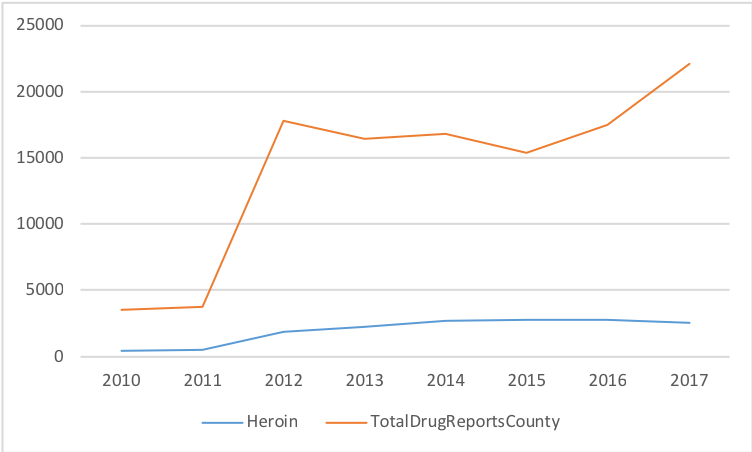
\includegraphics{figures/CUYAHOGACounty.png}
  \caption{Reports Graph of Ohio State Cuyahoga County}
\end{figure}




 
  \item 
According to our Drug Spread Model, we divided the drug abuse situation in each county into basic non-existence (A) existence (B) and serious existence (C) level 3 and simulated the states according to mathematical models.  The law of time and space changes in the number of cases in all counties.  We finally the following four conclusions
\begin{itemize}
  \item a)	
Grade A counties have a probability of 0.0277 and are converted to Grade B counties and it is almost impossible to directly convert to Grade A counties; Grade B counties have a 0.0365 chance to be converted to Grade A counties.
  \item b)	
If no policy intervention is added, some heavily drug-using counties in Ohio and Pennsylvania will be converted to moderate drug-using counties in the future and some moderate drug-drug counties in Kentucky, Virginia and West Virginia will be converted to severe drug-using counties. Therefore, the government should focus on drug cases in Kentucky Virginia and West Virginia.

  \item c)	
The number of counties in the three states of the five states tends to be stable over time, while Virginia is the first to reach a steady state, that is in the 60th year that is the drug identification in Virginia reached the threshold level in 2070.  

  \item d)	
It is worth mentioning that we have analyzed the number of heroin cases and found that the first case of heroin in Ohio began to occur. At the same time in the seventh year 2017 the heroin drug identification in Virginia reached the threshold level.
\end{itemize}

  \item 
Based on our research on socioeconomic data and the number of drug cases we have obtained 13 factors that may be closely related to the number of drug cases (see table below).  If you want to reduce the rate of drug abuse you can try to consider the development of relevant policies and laws and regulations from some aspects.
% Table generated by Excel2LaTeX from sheet 'Sheet1'
\begin{table}[htbp]
  \centering
  \caption{Factors that may be closely related to the number of drug cases}
  \small
    \begin{tabularx}{\textwidth}{c|X}
    \toprule
    1&HOUSEHOLDS BY TYPE - Total households - Family households (families) - Female householder, no husband present, family \\
    2&RESIDENCE 1 YEAR AGO - Population 1 year and over - Different house in the U.S. - Same county \\
    3&GRANDPARENTS - Number of grandparents living with own grandchildren under 18 years - Years responsible for grandchildren - 1 or 2 years \\
    4&ANCESTRY - Total population - Czech \\
    5&ANCESTRY - Total population - Dutch \\
    6&ANCESTRY - Total population - Scotch-Irish \\
    7&FERTILITY - Number of women 15 to 50 years old who had a birth in the past 12 months - Unmarried women (widowed, divorced, and never married) - Per 1,000 unmarried women \\
    8&EDUCATIONAL ATTAINMENT - Population 25 years and over - 9th to 12th grade, no diploma \\
    9&HOUSEHOLDS BY TYPE - Total households - Nonfamily households - Householder living alone \\
    10&ANCESTRY - Total population \\
    11&MARITAL STATUS - Females 15 years and over \\
    12&FERTILITY - Number of women 15 to 50 years old who had a birth in the past 12 months \\
    13&EDUCATIONAL ATTAINMENT - Population 25 years and over - Less than 9th grade \\
    \bottomrule
    \end{tabularx}%
  \label{tab:addlabel}%
\end{table}%




\end{enumerate}











































\newpage

















%
%
%\begin{itemize}
%\item \textbf{Applies widely}\\
%\cite{123ggplot2}
%This  system can be used for many types of airplanes, and it also
%solves the interference during  the procedure of the boarding
%airplane,as described above we can get to the  optimization
%boarding time.We also know that all the service is automate.
%\item \textbf{Improve the quality of the airport service}\\
%Balancing the cost of the cost and the benefit, it will bring in
%more convenient  for airport and passengers.It also saves many
%human resources for the airline. \item \textbf{}
%\end{itemize}
%
%
%
















































%
%
%\lipsum[8] \eqref{aa}
%\begin{equation}
%a^2 \label{aa}
%\end{equation}
%
% \begin{equation}
%  \begin{pmatrix}{*{20}c}
%  {a_{11} } & {a_{12} } & {a_{13} }  \\
%  {a_{21} } & {a_{22} } & {a_{23} }  \\
%  {a_{31} } & {a_{32} } & {a_{33} }  \\
%  \end{pmatrix}
%  = \frac{{Opposite}}{{Hypotenuse}}\cos ^{ - 1} \theta \arcsin \theta
% \end{equation}
%\lipsum[9]
%
% \begin{equation}
%  p_{j}=\begin{cases} 0,&\text{if $j$ is odd}\\
%  r!\,(-1)^{j/2},&\text{if $j$ is even}
%  \end{cases}
% \end{equation}
%
%\lipsum[10]
%
% \begin{equation}
%  \arcsin \theta  =
%  \mathop{{\int\!\!\!\!\!\int\!\!\!\!\!\int}\mkern-31.2mu
%  \bigodot}\limits_\varphi
%  {\mathop {\lim }\limits_{x \to \infty } \frac{{n!}}{{r!\left( {n - r}
%  \right)!}}} \eqno (1)
%\end{equation}
%

%\lipsum[11]
%
%\section{The Model Results}
%\lipsum[6]
%
%\section{Validating the Model}
%\lipsum[9]
%
%\section{Conclusions}
%\lipsum[6]
%
%\section{A Summary}
%\lipsum[6]
%
%\section{Evaluate of the Mode}
%
%\section{Strengths and weaknesses}
%\lipsum[12]

%\subsection{Strengths}
%\begin{itemize}
%\item \textbf{Applies widely}\\
%\cite{123ggplot2}
%This  system can be used for many types of airplanes, and it also
%solves the interference during  the procedure of the boarding
%airplane,as described above we can get to the  optimization
%boarding time.We also know that all the service is automate.
%\item \textbf{Improve the quality of the airport service}\\
%Balancing the cost of the cost and the benefit, it will bring in
%more convenient  for airport and passengers.It also saves many
%human resources for the airline. \item \textbf{}
%\end{itemize}

%\begin{thebibliography}{99}
%\bibitem{1} D.~E. KNUTH   The \TeX{}book  the American
%Mathematical Society and Addison-Wesley
%Publishing Company , 1984-1986.
%\bibitem{2}Lamport, Leslie,  \LaTeX{}: `` A Document Preparation System '',
%Addison-Wesley Publishing Company, 1986.
%\bibitem{3}\url{http://www.latexstudio.net/}
%\bibitem{4}\url{http://www.chinatex.org/}
%
%\end{thebibliography}
\bibliographystyle{plain}

\bibliography{ref}



\begin{appendices}


\section{Percent Margin Error Data and Variable Graph}\label{Percent Margin Error Data and Variable Graph}
After the analysis of 2010, we have done the same analysis to the data from 2011 to 2016, and draw the following pictures.
\begin{figure}[H]
\centering
\begin{minipage}[t]{0.45\textwidth}
\centering
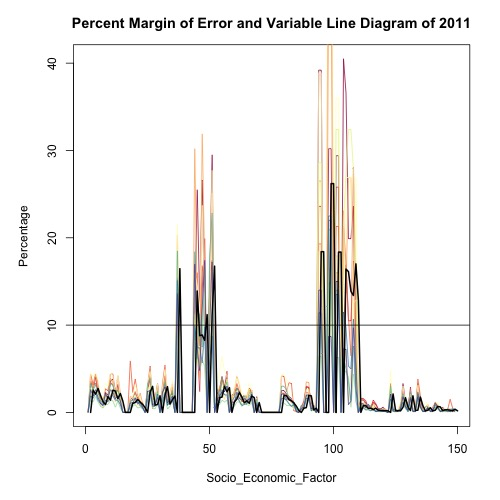
\includegraphics[width=3.2in]{figures/PercentMarginErrorDataGraphVariable2011.jpeg}
\caption{Percent Margin Error Data and Variable Graph 2011}
\label{Percent Margin Error Data and Variable Graph 2011}
\end{minipage}
\hfill
\begin{minipage}[t]{0.45\textwidth}
\centering
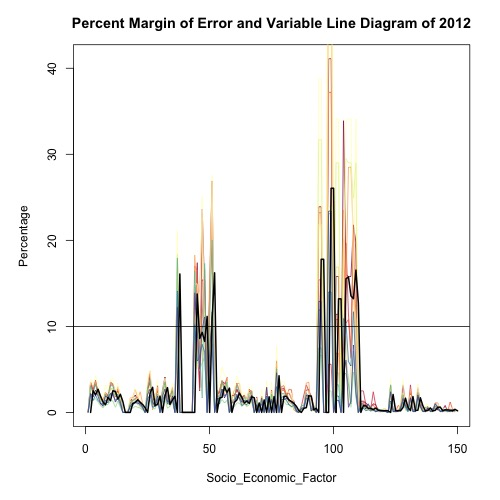
\includegraphics[width=3.2in]{figures/PercentMarginErrorDataGraphVariable2012.jpeg}
\caption{Percent Margin Error Data and Variable Graph 2012}
\label{Percent Margin Error Data and Variable Graph 2012}
\end{minipage}
\end{figure}

\begin{figure}[H]
\centering
\begin{minipage}[t]{0.45\textwidth}
\centering
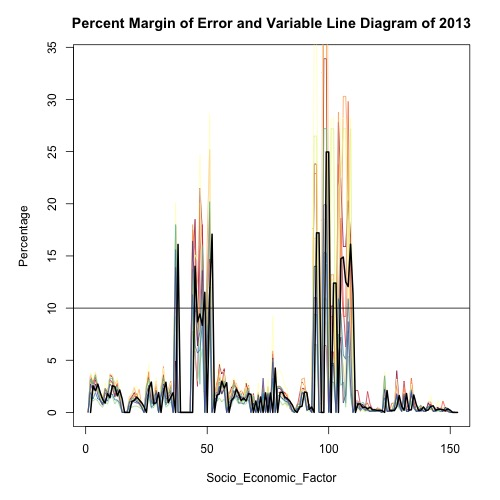
\includegraphics[width=3.2in]{figures/PercentMarginErrorDataGraphVariable2013.jpeg}
\caption{Percent Margin Error Data and Variable Graph 2013}
\label{Percent Margin Error Data and Variable Graph 2013}
\end{minipage}
\hfill
\begin{minipage}[t]{0.45\textwidth}
\centering
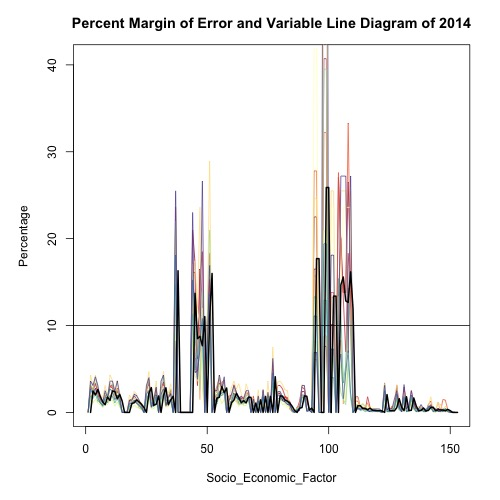
\includegraphics[width=3.2in]{figures/PercentMarginErrorDataGraphVariable2014.jpeg}
\caption{Percent Margin Error Data and Variable Graph 2014}
\label{Percent Margin Error Data and Variable Graph 2014}
\end{minipage}
\end{figure}

\begin{figure}[H]
\centering
\begin{minipage}[t]{0.45\textwidth}
\centering
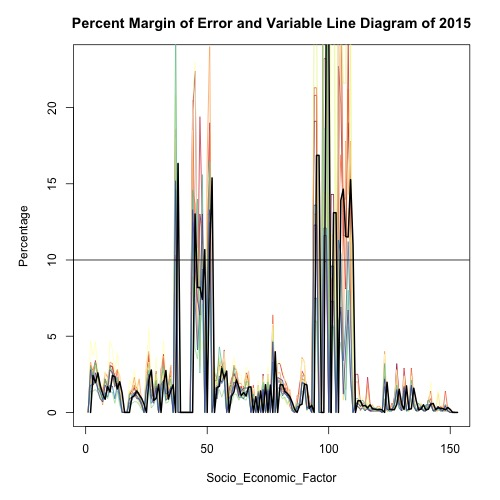
\includegraphics[width=3.2in]{figures/PercentMarginErrorDataGraphVariable2015.jpeg}
\caption{Percent Margin Error Data and Variable Graph 2015}
\label{Percent Margin Error Data and Variable Graph 2015}
\end{minipage}
\hfill
\begin{minipage}[t]{0.45\textwidth}
\centering
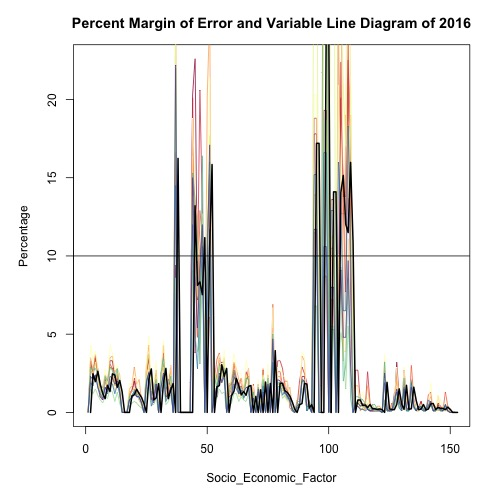
\includegraphics[width=3.2in]{figures/PercentMarginErrorDataGraphVariable2016.jpeg}
\caption{Percent Margin Error Data and Variable Graph 2016}
\label{Percent Margin Error Data and Variable Graph 2016}
\end{minipage}
\end{figure}


\section{Changes of Interpretation Variable and Coefficients Graph in LASSO Regression}\label{Changes of Interpretation Variable and Coefficients Graph in LASSO Regression}

\begin{figure}[H]
\centering
\begin{minipage}[t]{0.45\textwidth}
\centering
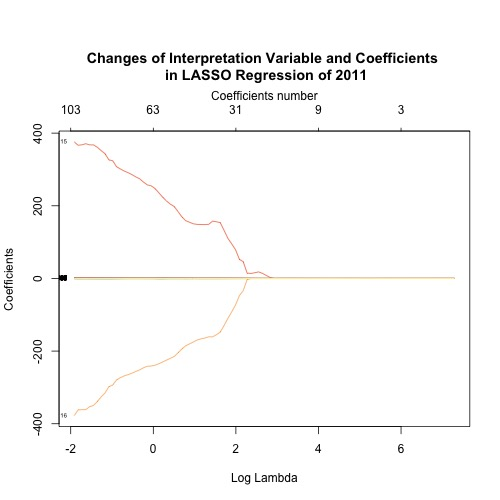
\includegraphics[width=3.2in]{figures/ChangesofInterpretationVariableandCoefficientsinLASSORegressionof2011.jpeg}
\caption{Changes of Interpretation Variable and Coefficients Graph in LASSO Regression of 2011}
\label{Changes of Interpretation Variable and Coefficients Graph in LASSO Regression of 2011}
\end{minipage}
\hfill
\begin{minipage}[t]{0.45\textwidth}
\centering
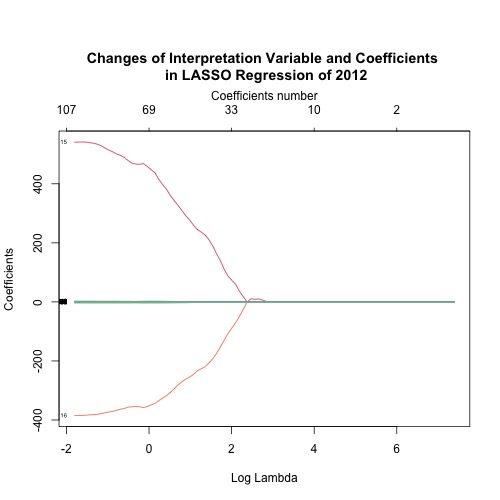
\includegraphics[width=3.2in]{figures/ChangesofInterpretationVariableandCoefficientsinLASSORegressionof2012.jpeg}
\caption{Changes of Interpretation Variable and Coefficients Graph in LASSO Regression of 2012}
\label{Changes of Interpretation Variable and Coefficients Graph in LASSO Regression of 2012}
\end{minipage}
\end{figure}

\begin{figure}[H]
\centering
\begin{minipage}[t]{0.45\textwidth}
\centering
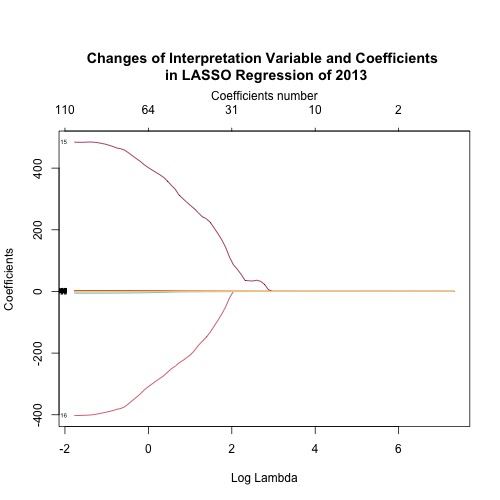
\includegraphics[width=3.2in]{figures/ChangesofInterpretationVariableandCoefficientsinLASSORegressionof2013.jpeg}
\caption{Changes of Interpretation Variable and Coefficients Graph in LASSO Regression of 2013}
\label{Changes of Interpretation Variable and Coefficients Graph in LASSO Regression of 2013}
\end{minipage}
\hfill
\begin{minipage}[t]{0.45\textwidth}
\centering
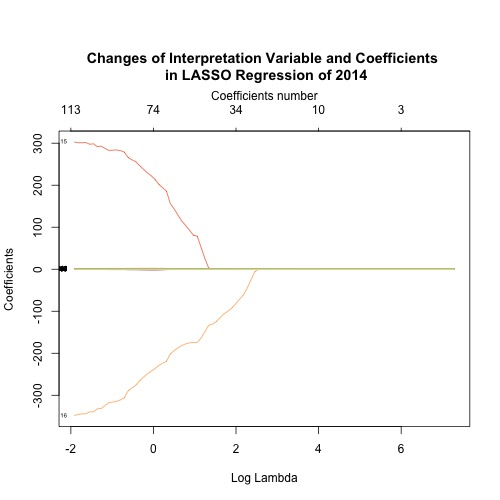
\includegraphics[width=3.2in]{figures/ChangesofInterpretationVariableandCoefficientsinLASSORegressionof2014.jpeg}
\caption{Changes of Interpretation Variable and Coefficients Graph in LASSO Regression of 2014}
\label{Changes of Interpretation Variable and Coefficients Graph in LASSO Regression of 2014}
\end{minipage}
\end{figure}

\begin{figure}[H]
\centering
\begin{minipage}[t]{0.45\textwidth}
\centering
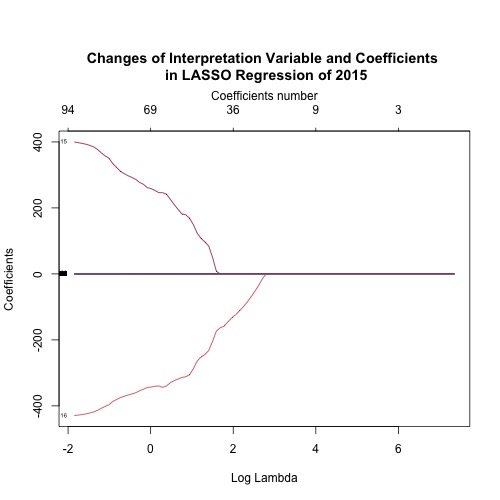
\includegraphics[width=3.2in]{figures/ChangesofInterpretationVariableandCoefficientsinLASSORegressionof2015.jpeg}
\caption{Changes of Interpretation Variable and Coefficients Graph in LASSO Regression of 2015}
\label{Changes of Interpretation Variable and Coefficients Graph in LASSO Regression of 2015}
\end{minipage}
\hfill
\begin{minipage}[t]{0.45\textwidth}
\centering
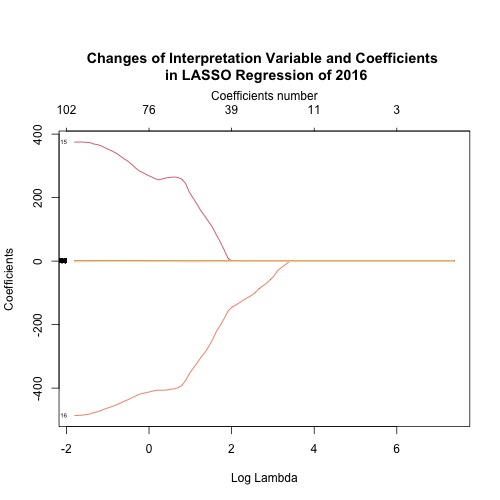
\includegraphics[width=3.2in]{figures/ChangesofInterpretationVariableandCoefficientsinLASSORegressionof2016.jpeg}
\caption{Changes of Interpretation Variable and Coefficients Graph in LASSO Regression of 2016}
\label{Changes of Interpretation Variable and Coefficients Graph in LASSO Regression of 2016}
\end{minipage}
\end{figure}


\section{Total Drug Reports County}\label{Total Drug Reports County}

\begin{figure}[H]
\centering
\begin{minipage}[t]{0.45\textwidth}
\centering
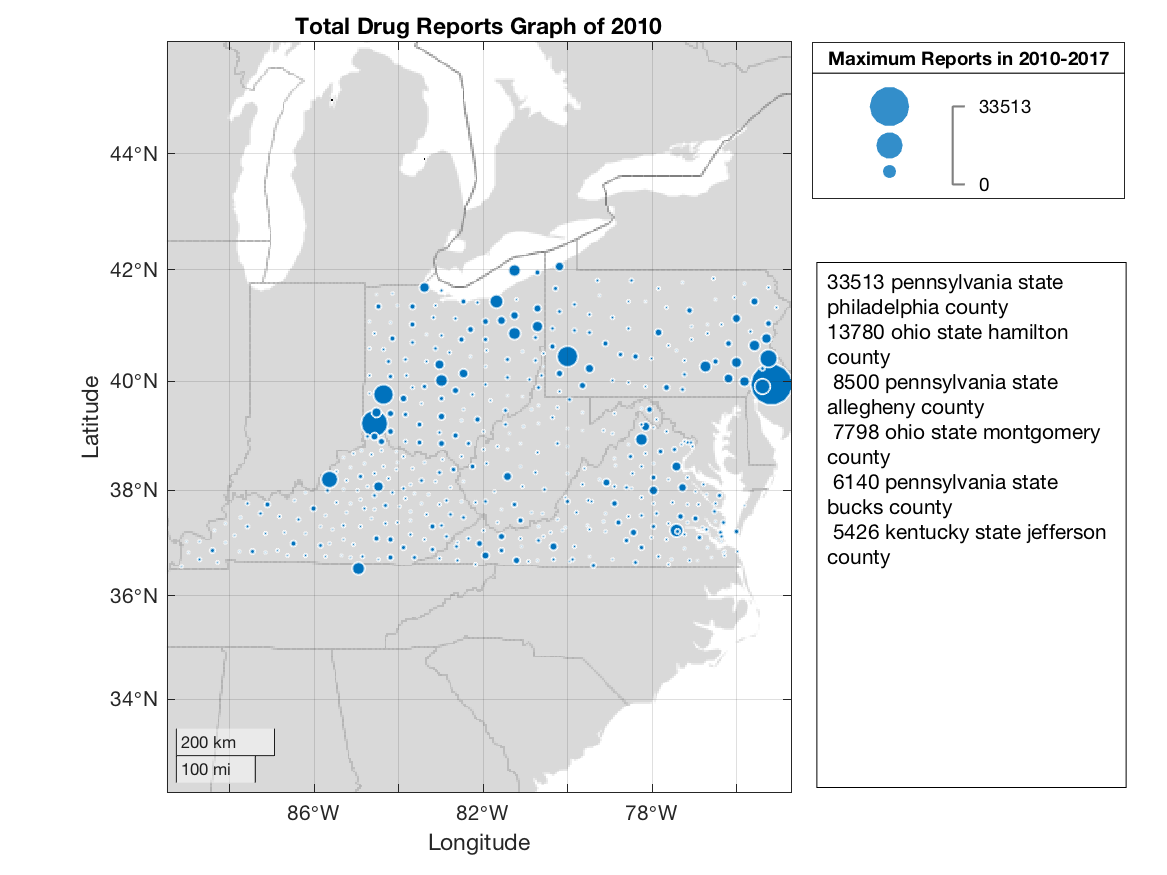
\includegraphics[width=3.2in]{figures/TotalDrugReportsCounty2010.png}
\caption{Total Drug Reports County in 2010}
\label{Total Drug Reports County in 2010}
\end{minipage}
\hfill
\begin{minipage}[t]{0.45\textwidth}
\centering
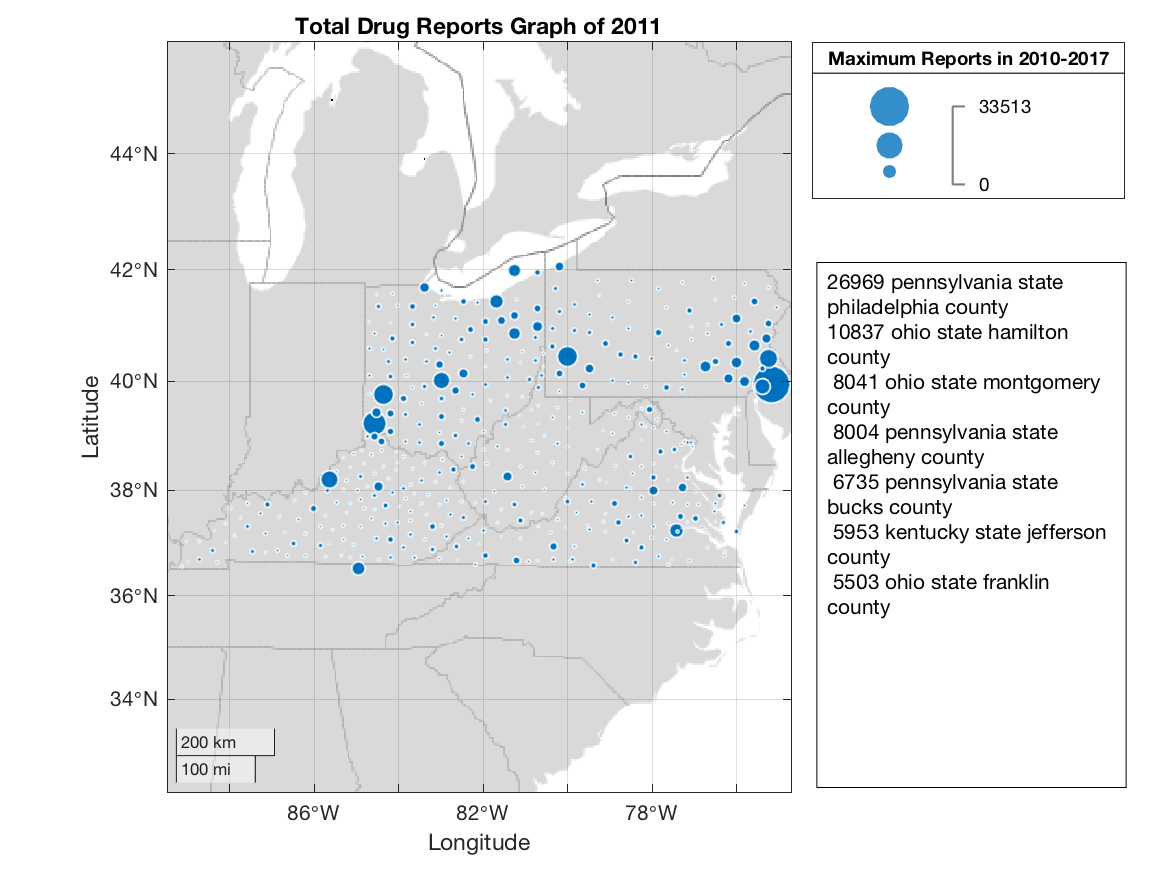
\includegraphics[width=3.2in]{figures/TotalDrugReportsCounty2011.png}
\caption{Total Drug Reports County in 2011}
\label{Total Drug Reports County in 2011}
\end{minipage}
\end{figure}

\begin{figure}[H]
\centering
\begin{minipage}[t]{0.45\textwidth}
\centering
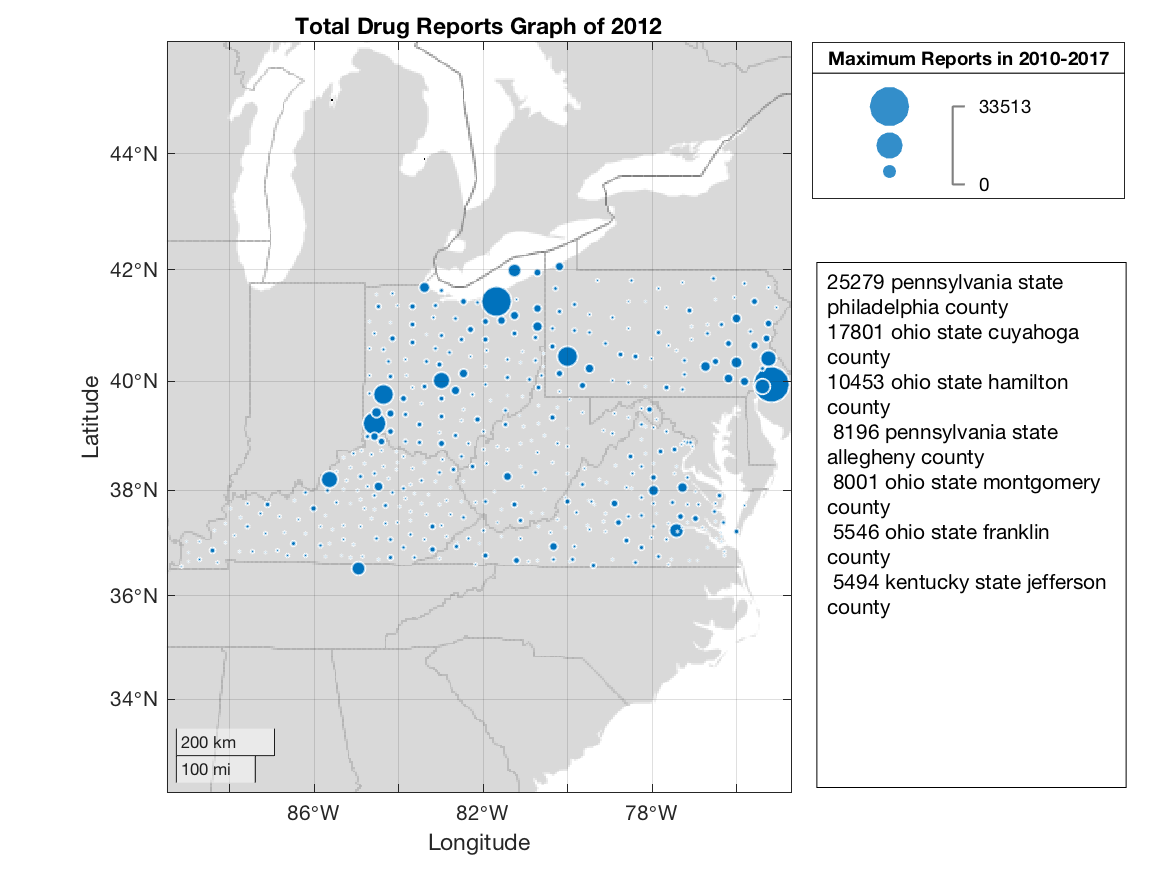
\includegraphics[width=3.2in]{figures/TotalDrugReportsCounty2012.png}
\caption{Total Drug Reports County in 2012}
\label{Total Drug Reports County in 2012}
\end{minipage}
\hfill
\begin{minipage}[t]{0.45\textwidth}
\centering
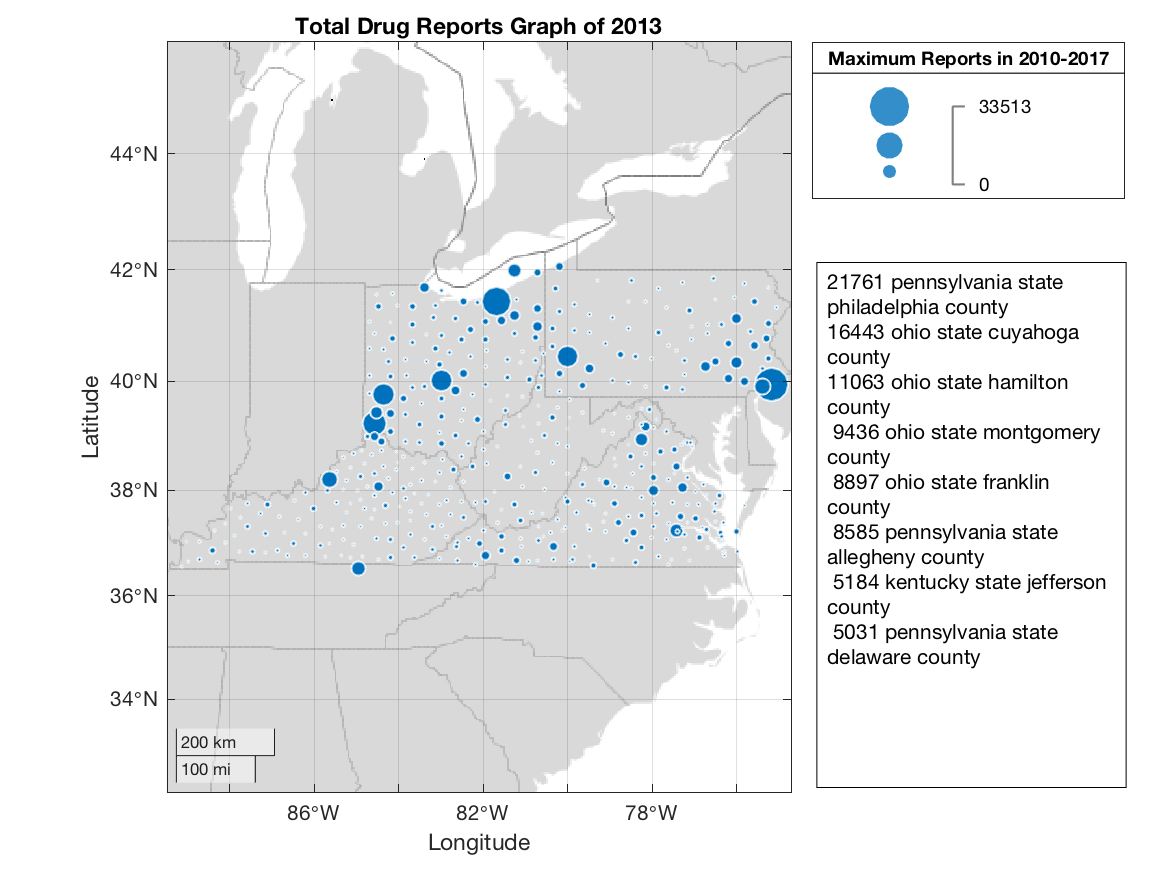
\includegraphics[width=3.2in]{figures/TotalDrugReportsCounty2013.png}
\caption{Total Drug Reports County in 2013}
\label{Total Drug Reports County in 2013}
\end{minipage}
\end{figure}

\begin{figure}[H]
\centering
\begin{minipage}[t]{0.45\textwidth}
\centering
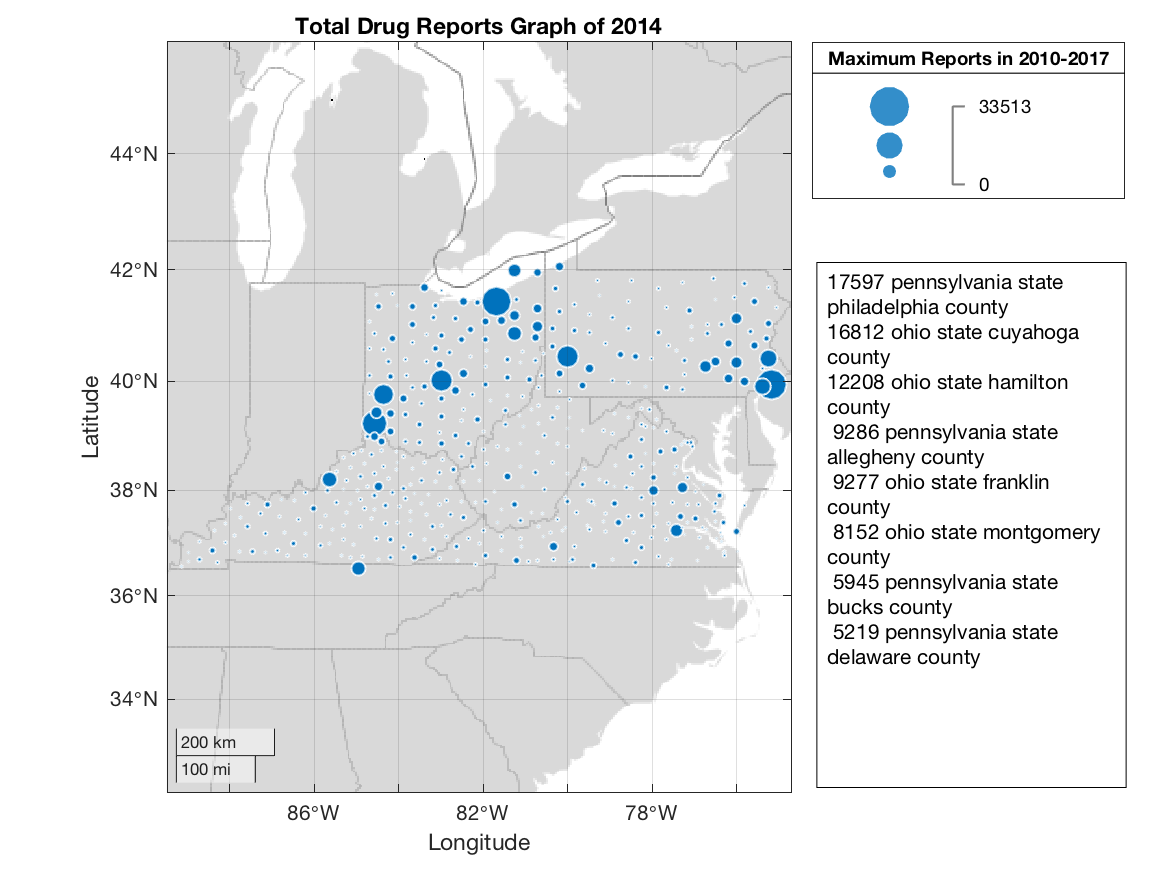
\includegraphics[width=3.2in]{figures/TotalDrugReportsCounty2014.png}
\caption{Total Drug Reports County in 2014}
\label{Total Drug Reports County in 2014}
\end{minipage}
\hfill
\begin{minipage}[t]{0.45\textwidth}
\centering
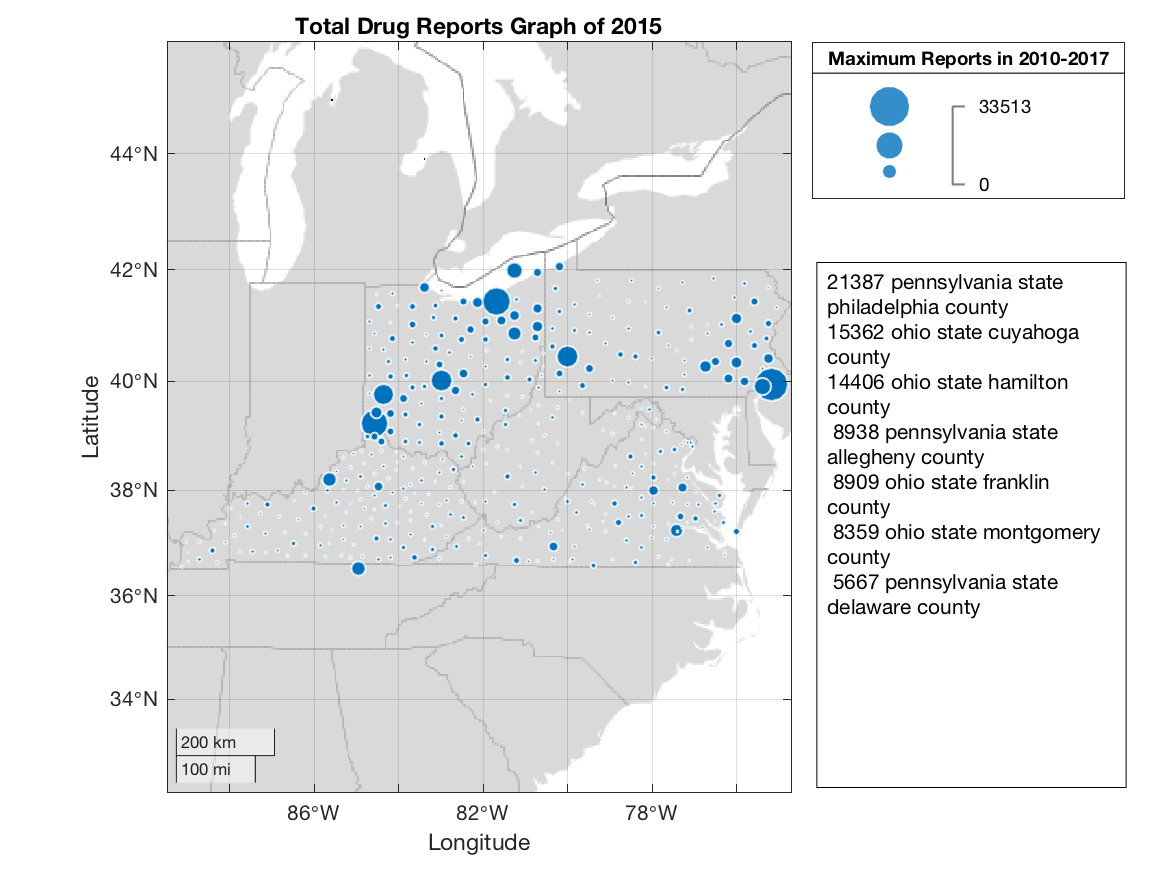
\includegraphics[width=3.2in]{figures/TotalDrugReportsCounty2015.png}
\caption{Total Drug Reports County in 2015}
\label{Total Drug Reports County in 2015}
\end{minipage}
\end{figure}











\section{Matlab Code}\label{Matlab Code}

Here are simulation programmes we used in our model as follow.\\

\textbf{\textcolor[rgb]{0.98,0.00,0.00}{Input matlab source:}}
\lstinputlisting[language=Matlab]{./code/test.m}
\lstinputlisting[language=Matlab]{./code/geoCode.m}
\lstinputlisting[language=Matlab]{./code/geoDist.m}
\lstinputlisting[language=Matlab]{./code/createfigure.m}




\section{R Code}\label{R Code}

Here are simulation programmes we used in our model as follow.\\

\textcolor[rgb]{0.98,0.00,0.00}{\textbf{Input R source:}}
\lstinputlisting[language=R]{./code/Lassotest.R}

\end{appendices}
\end{document}

%%
%% This work consists of these files mcmthesis.dtx,
%%                                   figures/ and
%%                                   code/,
%% and the derived files             mcmthesis.cls,
%%                                   mcmthesis-demo.tex,
%%                                   README,
%%                                   LICENSE,
%%                                   mcmthesis.pdf and
%%                                   mcmthesis-demo.pdf.
%%
%% End of file `mcmthesis-demo.tex'.
